\documentclass[a4paper,10pt,titlepage]{article}

\usepackage[utf8]{inputenc}

\usepackage[pdftex]{hyperref}
\hypersetup{
colorlinks = true,
linkcolor = black,
}
\usepackage{graphicx}

\author{Binary Ninjaz}
\title{Harvest Website Manual}
\date{}

\begin{document}
\maketitle
\pagenumbering{Roman}
\tableofcontents
\newpage
\listoffigures
\newpage
\pagenumbering{arabic}
\section{Use}
\subsection{Getting Started}
\subsubsection{Resigtering}
\paragraph{Finding the Register Page}The registration page can be found at <Web Link>, and once there the user will be presented with the page as seen in \ref{RegisterPage}. It is important to note that the login page can also be accessed from \ref{LoginPage} by clicking on the \texttt{Sign Up} button at the top left of the page, or by clicking on the blue \texttt{Create New Account} button.

\begin{figure}
 \centering
 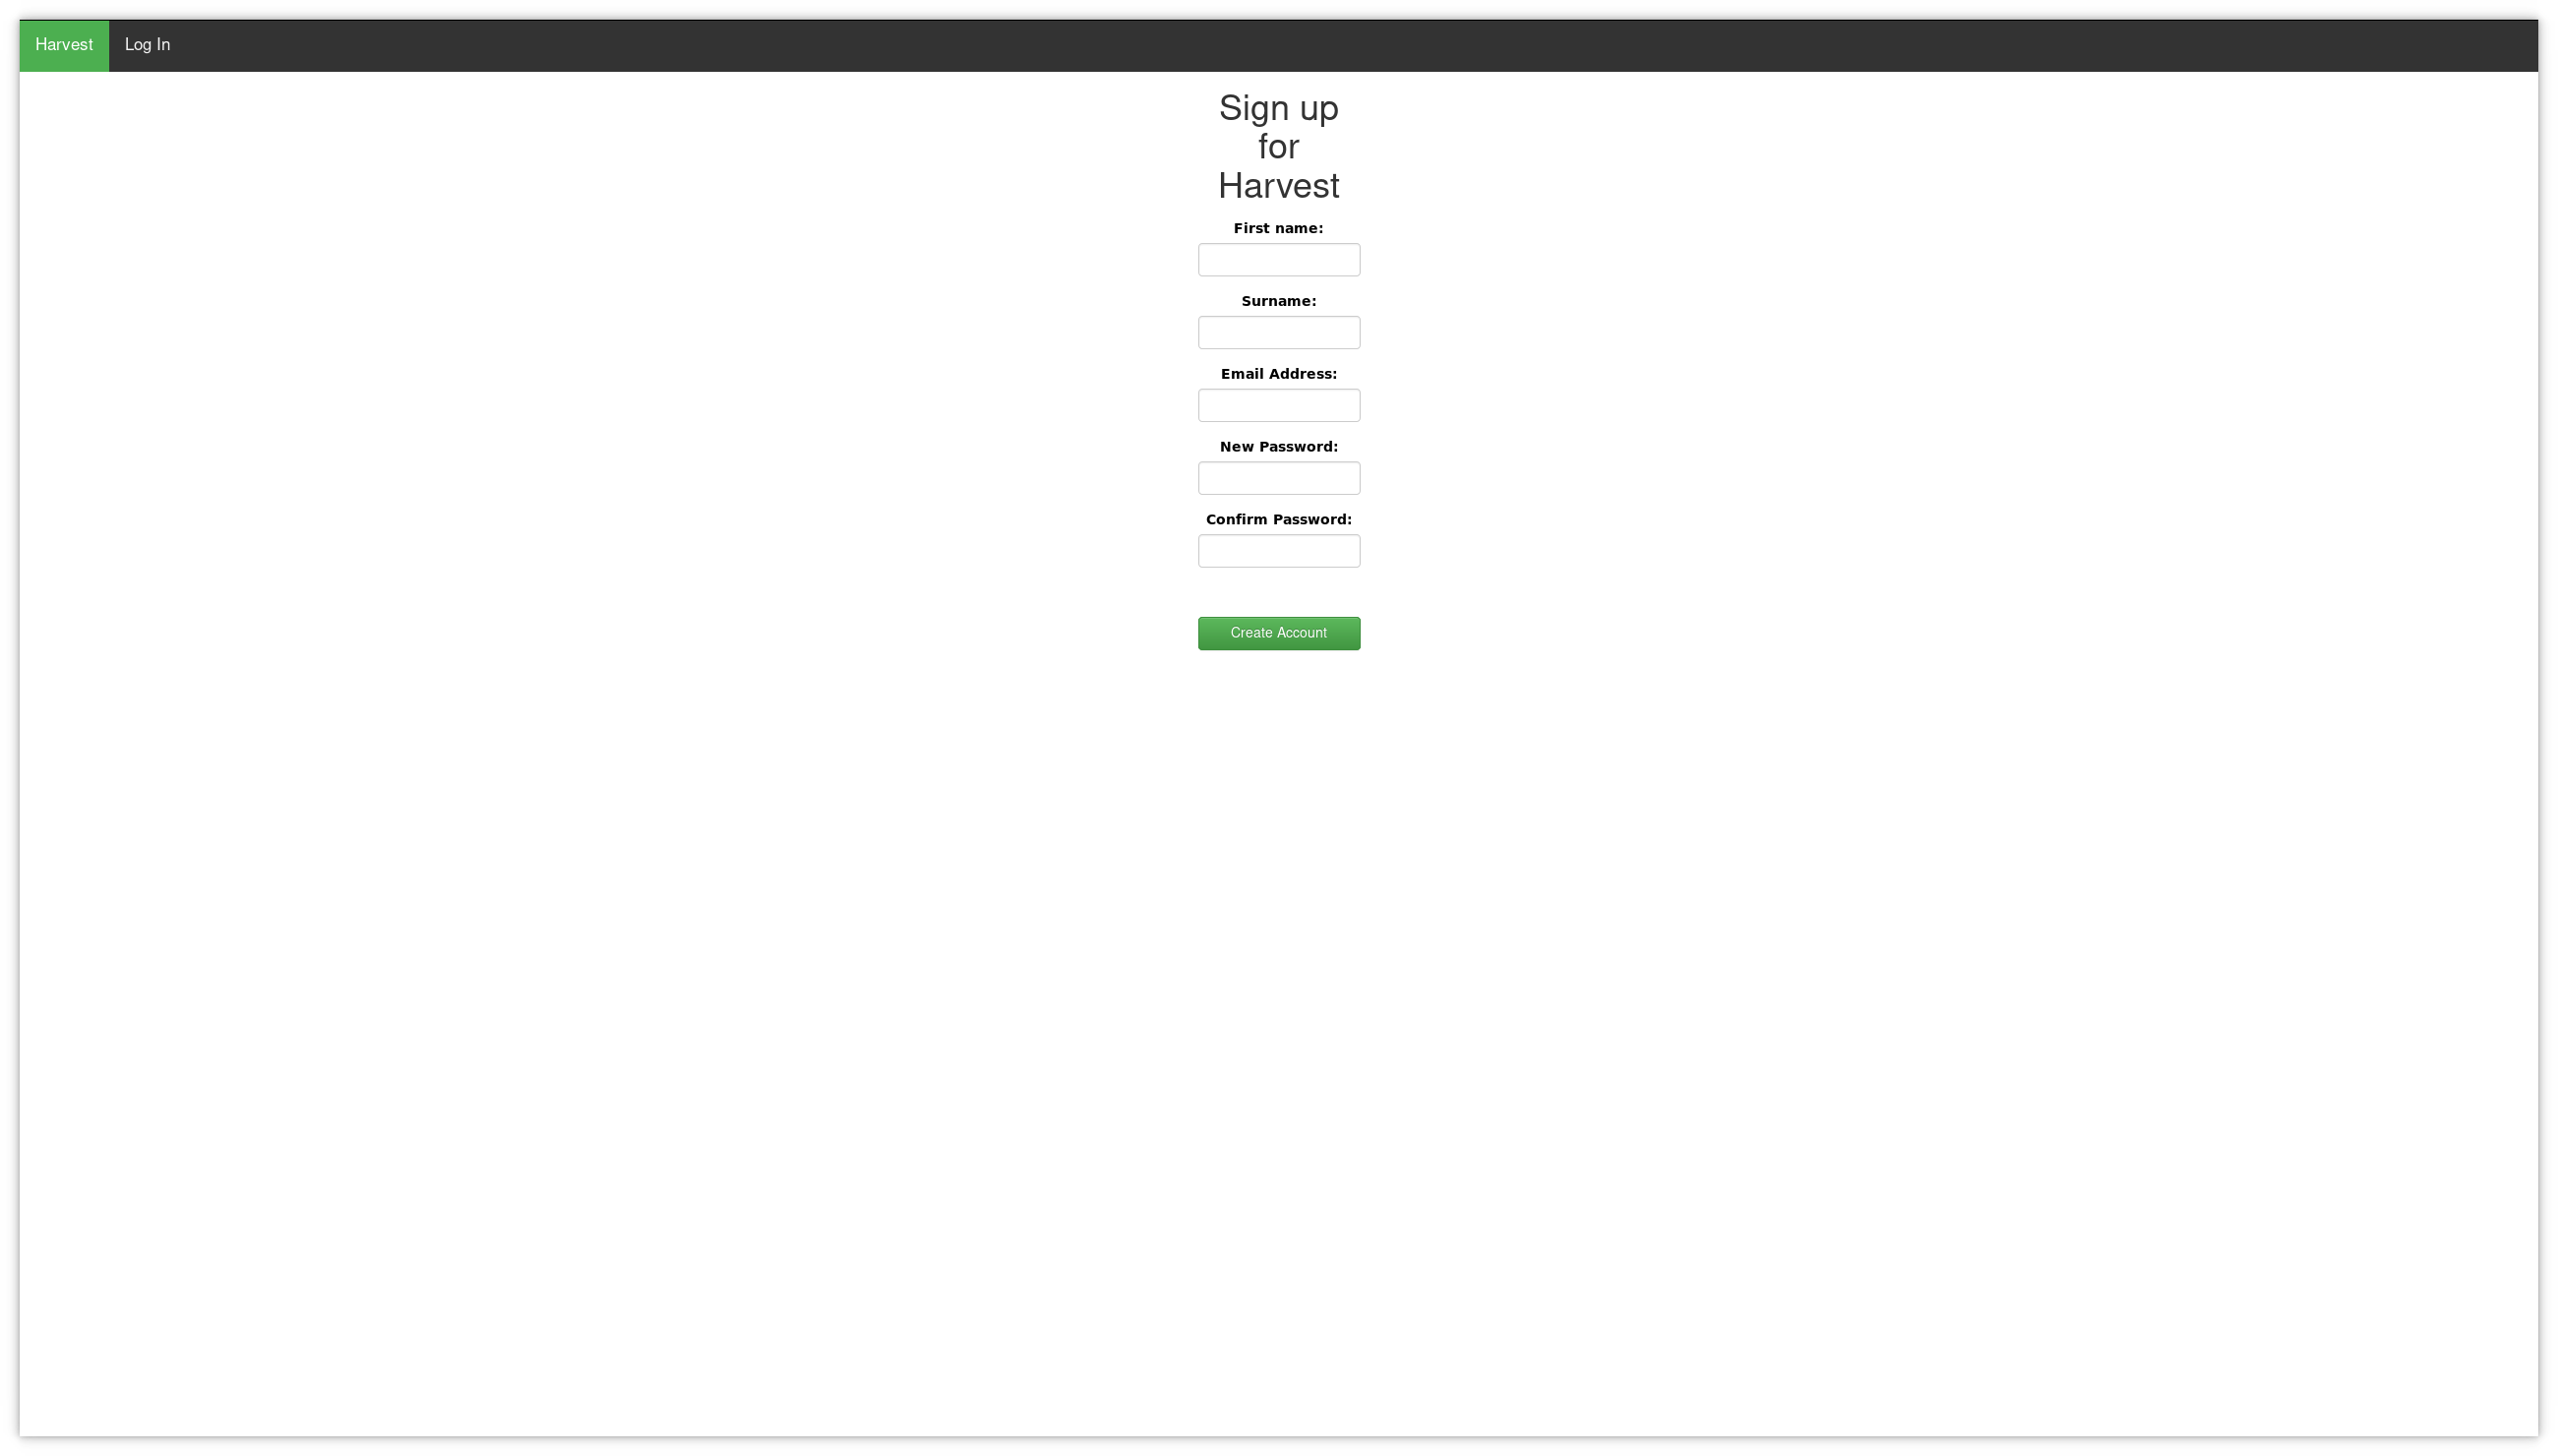
\includegraphics[width=12cm, keepaspectratio]{Images/Register-Page.png}
 % Screenshot_20180407_191730.png: 2600x1480 px, 121dpi, 54.58x31.07 cm, bb=0 0 1547 881
 \caption{Register Page}
 \label{RegisterPage}
\end{figure}

\paragraph{Creating an Account}Once at the register page the new user must enter their first name, surname, email address, desired password, and confirm the desired password by entering it again. When all of the information has been entered, and the user is content that the information is correct, they shall click on the green \texttt{Create Account} button. They will now be taken to the login page as seen in \ref{LoginPage}. The user shall receive an email as seen in \ref{AccountCreationConfirmationEmail} at the specified address, asking to confirm their account. The user simply needs to click on the \texttt{Confirm Account} button in order to complete the account creation.

\subsubsection{Logging In}
\paragraph{Finding the Login Page}The login page can be found at <Web Link>, and once there the user will be presented with the page as seen in \ref{LoginPage}. It is important to note that the login page can also be accessed from \ref{RegisterPage} by clicking on the \texttt{Log In} button at the top left of the page.

\begin{figure}
 \centering
 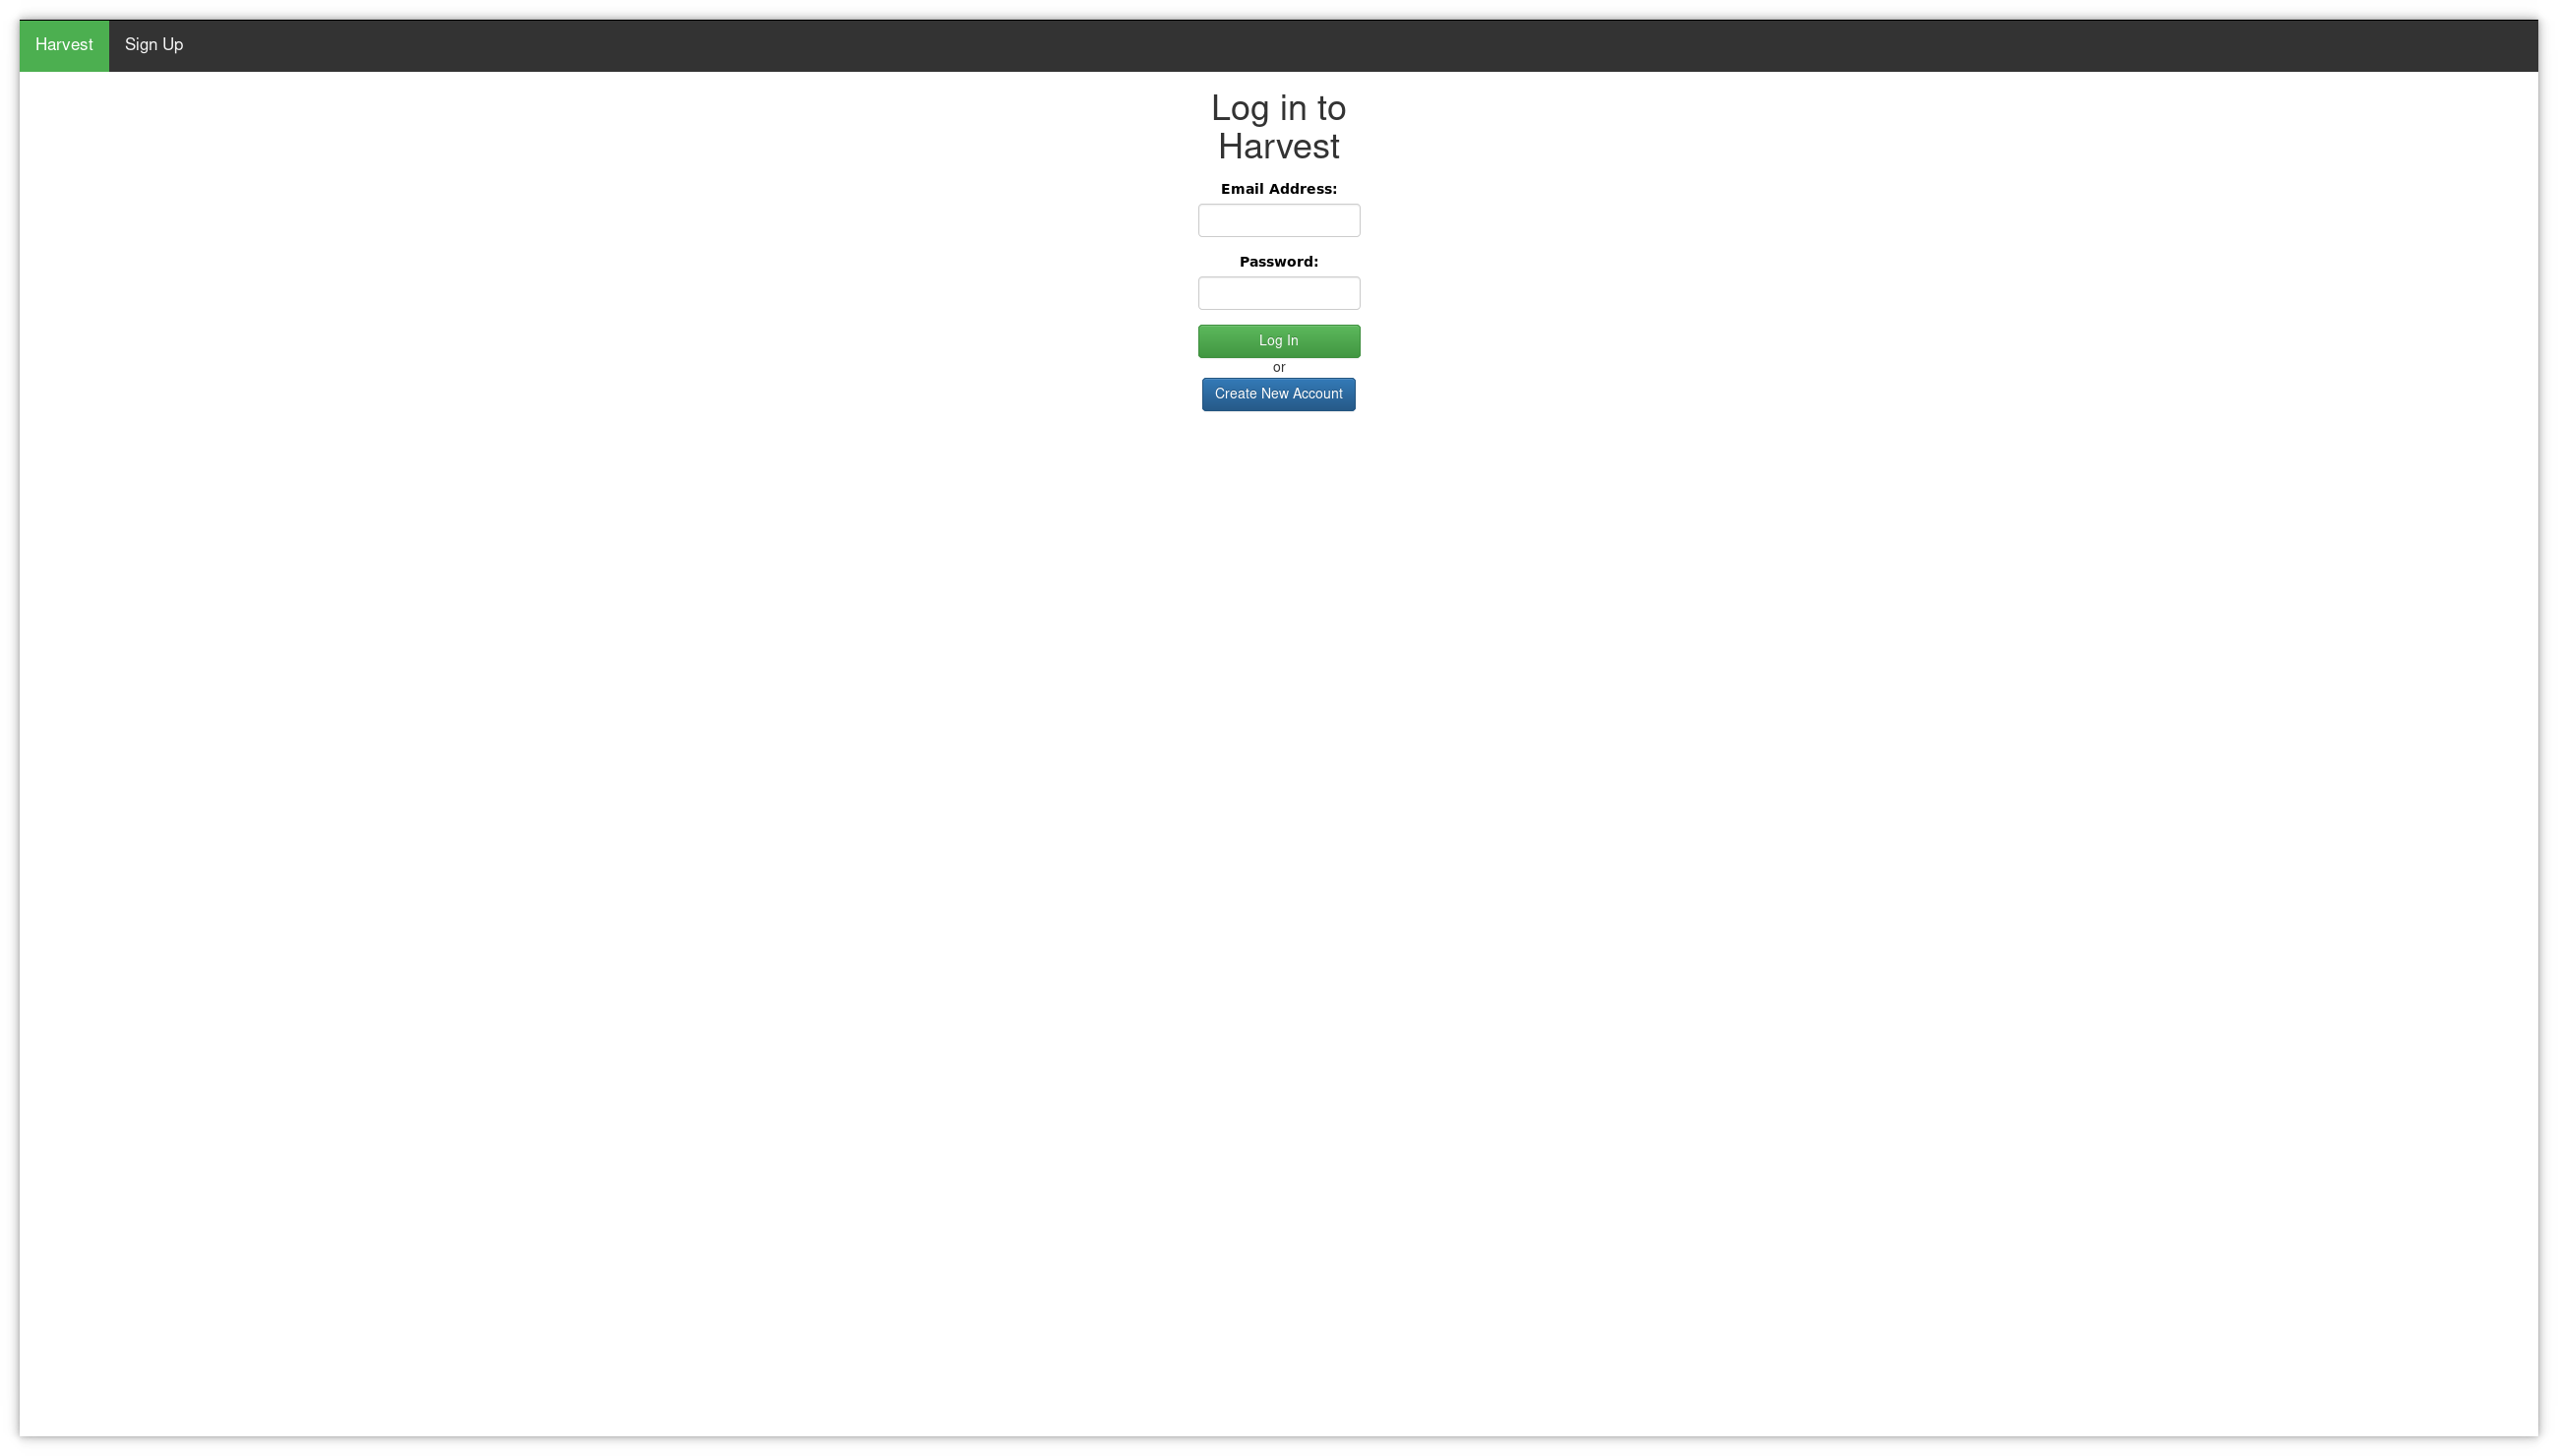
\includegraphics[width=12cm, keepaspectratio]{Images/Login-Page.png}
 % Screenshot_20180407_191730.png: 2600x1480 px, 121dpi, 54.58x31.07 cm, bb=0 0 1547 881
 \caption{Login Page}
 \label{LoginPage}
\end{figure}

\paragraph{Logging In}The user simply enters the correct email address and password associated with their account, and clicks on the green \texttt{Log In} button. The user will the now be taken to \ref{HomePage}.

\subsubsection{Home Page}
Once the user has logged in, they will be taken to the home page, as seen in \ref{HomePage}. The home page is the starting point of the system, it serves simply by providing a real time updating feed of all bag drops.

\subsubsection{Universal Features}
Once the user is logged in, all web pages follow a similar design, so that use is consistent and manageable. The navbar that appears at the top of all logged in screens is consistent. Buttons in the navbar, from left to right are (note that the active page is always highlighted in green): 
\paragraph{Harvest Home}Takes the user to the home page, as seen in \ref{HomePage}.
\paragraph{View/Edit Information}Takes the user to the View/Edit Information page, as seen in \ref{InformationPage}.
\paragraph{Sign Out}Logs the user out of the system, and returns them to the login page, as seen in \ref{LoginPage}

\begin{figure}
 \centering
 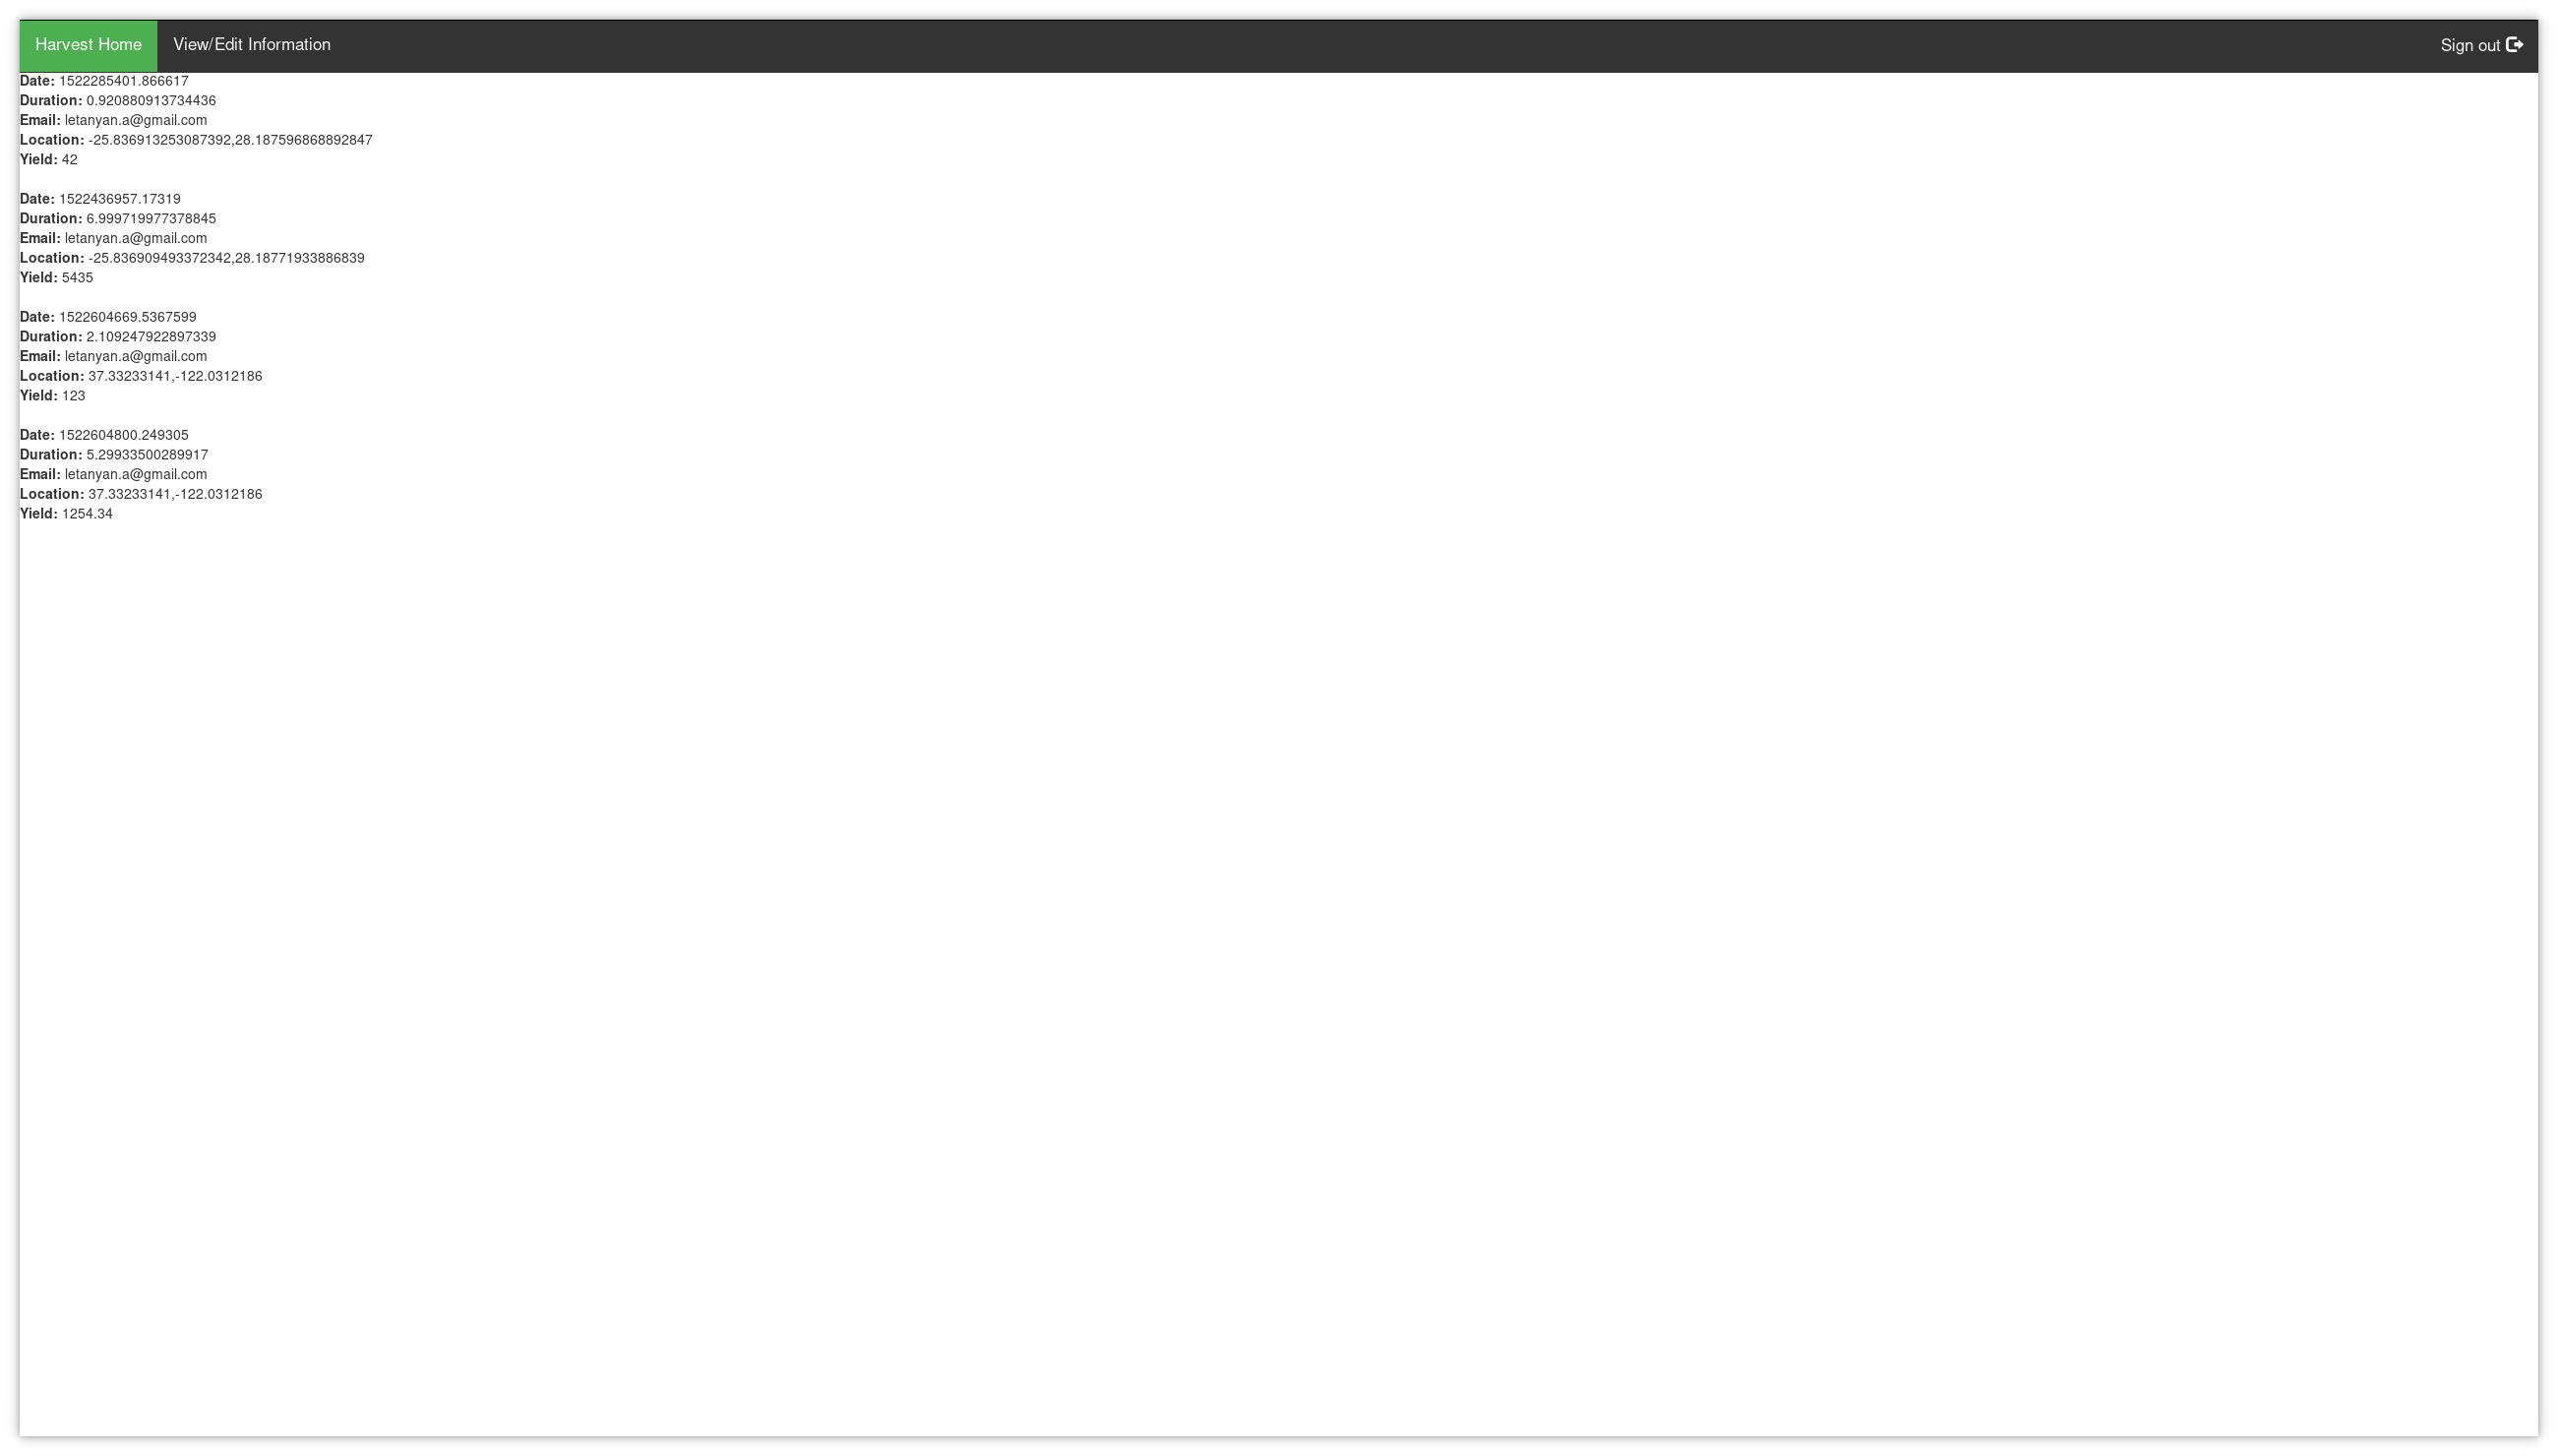
\includegraphics[width=12cm, keepaspectratio]{Images/Home-Page.png}
 % Screenshot_20180407_191730.png: 2600x1480 px, 121dpi, 54.58x31.07 cm, bb=0 0 1547 881
 \caption{Home Page}
 \label{HomePage}
\end{figure}

\subsection{View/Edit Information}
\paragraph{Introduction}The View/Edit Information page can be found at any time by clicking on the \texttt{View/Edit Information} button in the navbar. Once clicked on, the user will be taken to \ref{InformationPage}. The concept is that almost all information can be viewed from this page, and once the relevant information has been located, it can also be edited.

\begin{figure}
 \centering
 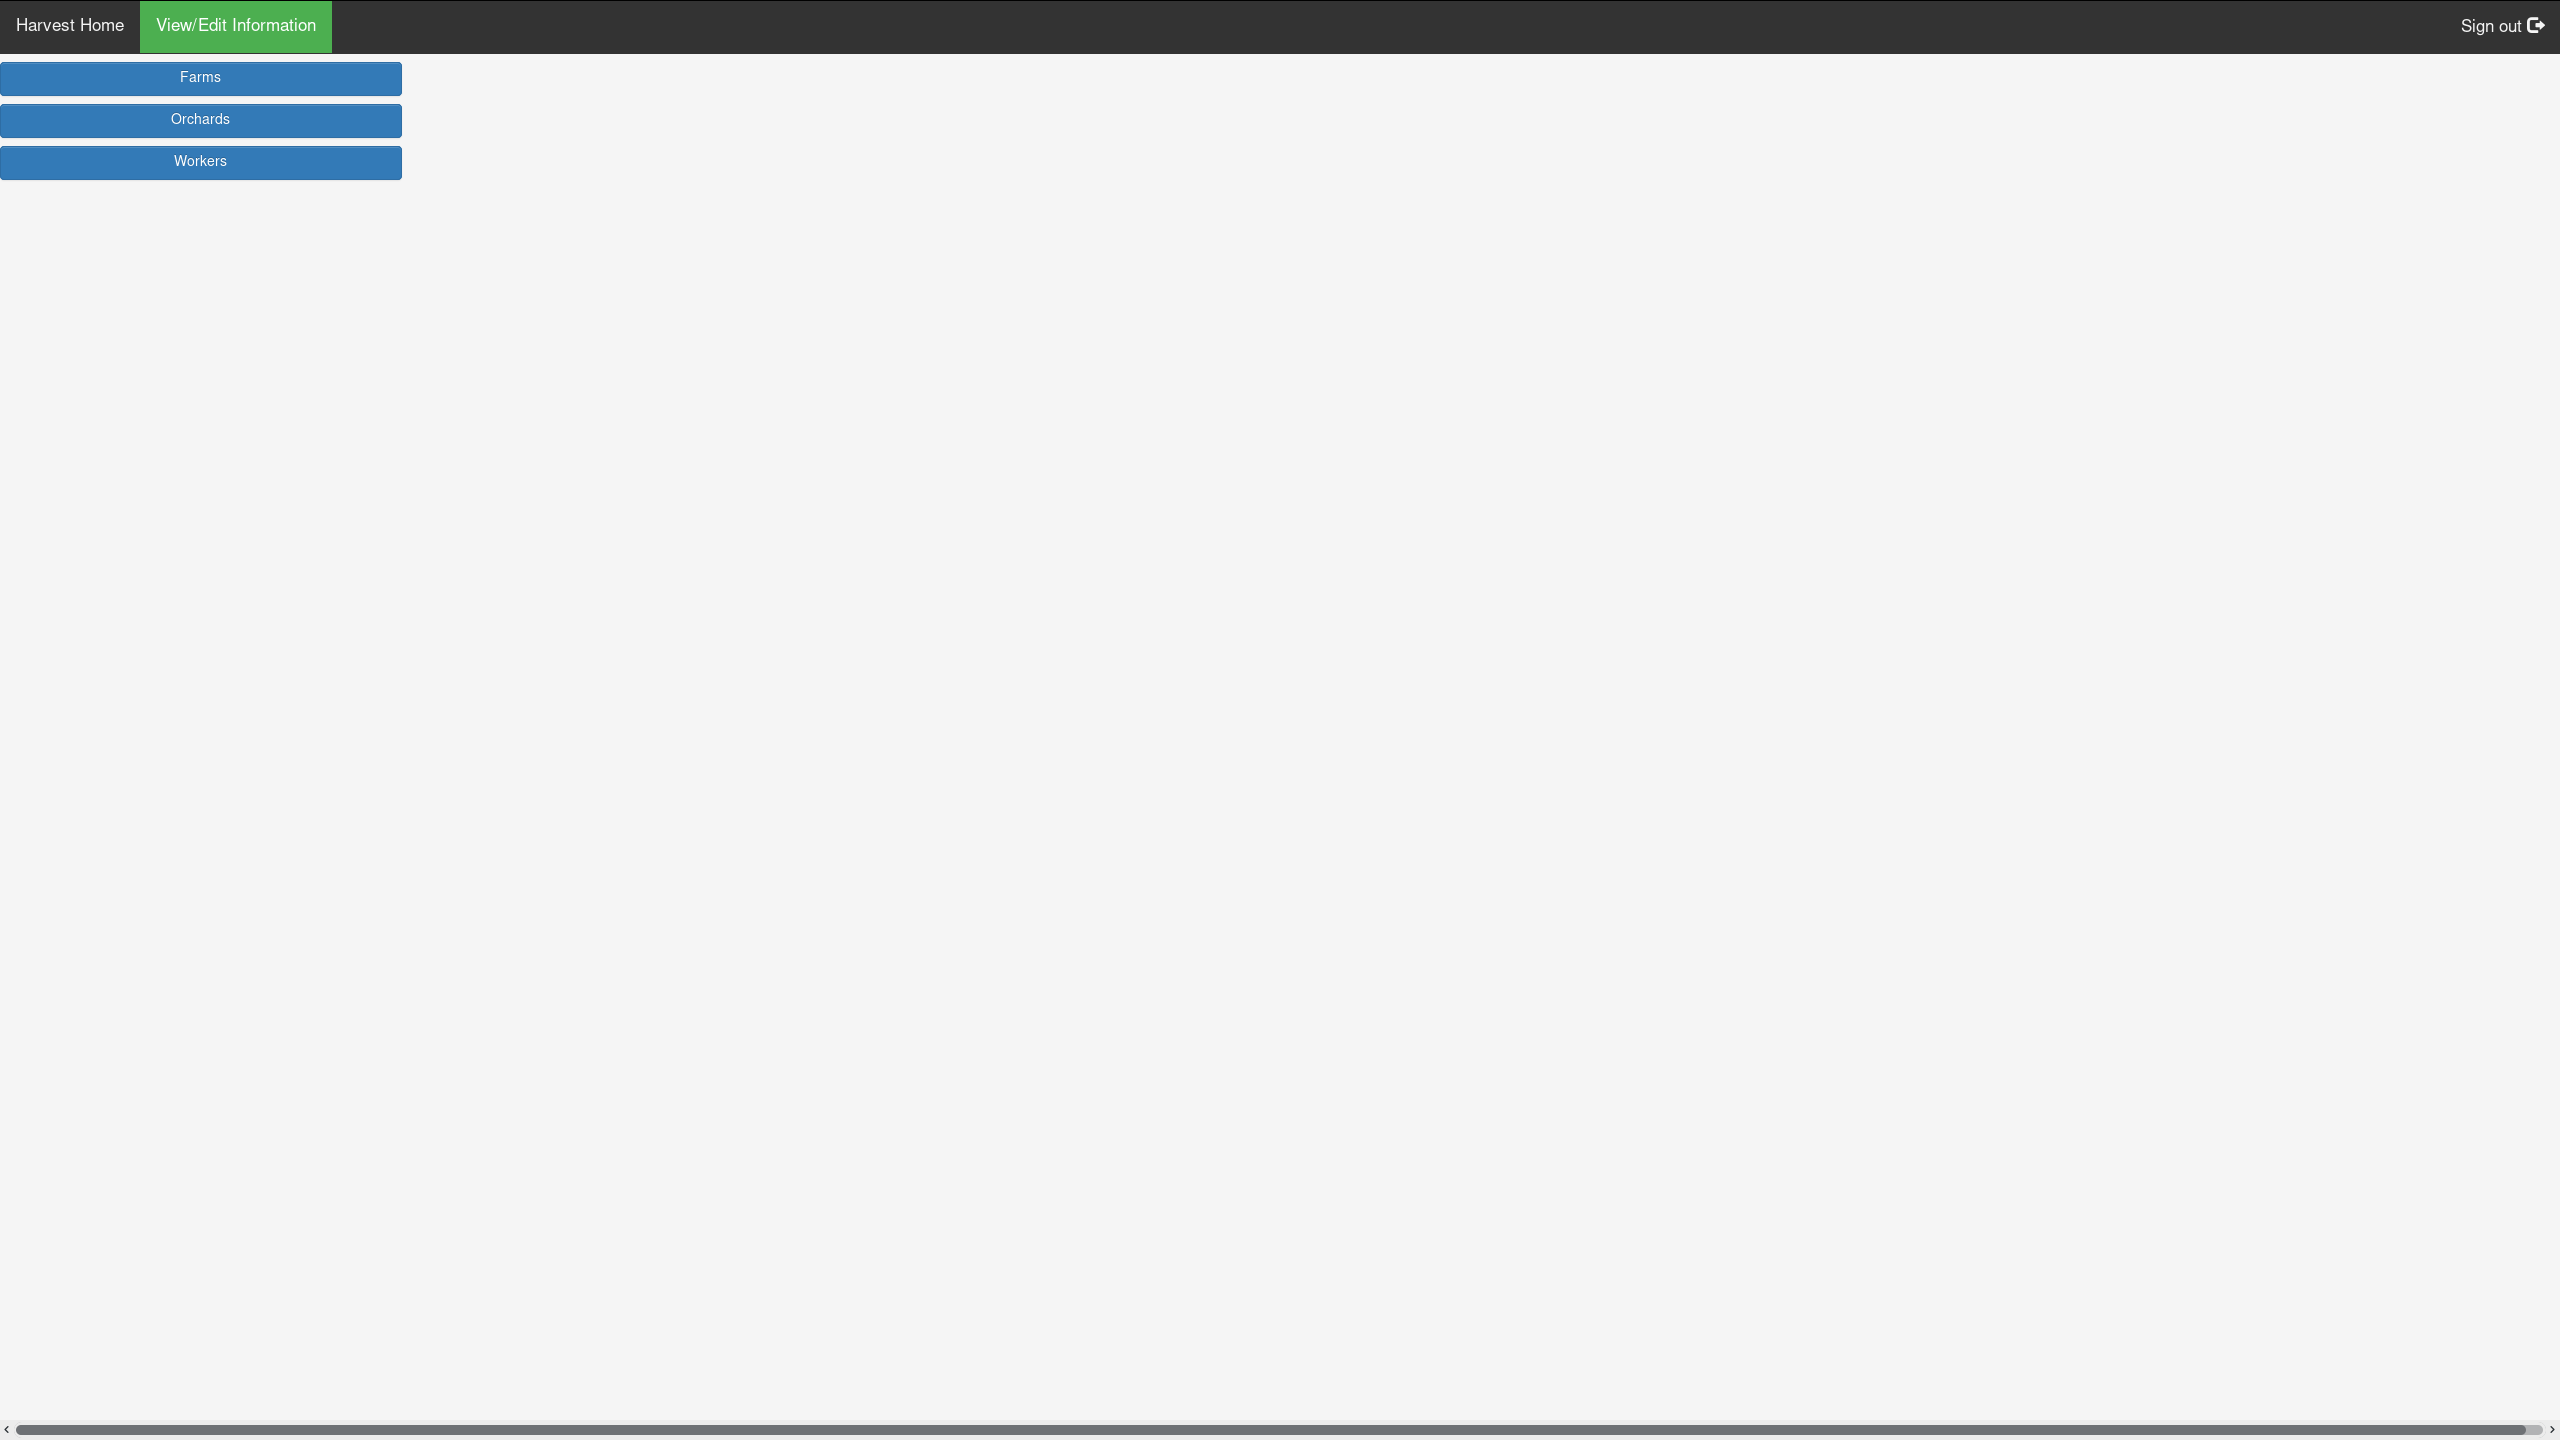
\includegraphics[width=12cm, keepaspectratio]{Images/Information-Page.png}
 % Screenshot_20180407_191730.png: 2600x1480 px, 121dpi, 54.58x31.07 cm, bb=0 0 1547 881
 \caption{View/Edit Information Page}
 \label{InformationPage}
\end{figure}

\paragraph{Locating the Correct Information}When in \ref{InformationPage} there are three blue buttons available; \texttt{Farms}, \texttt{Orchards}, and \texttt{Workers}. Each of which will expand a list of the relevant items. The entire process is best described through an example, so, in this example, the goal is to locate information on a worker named \textit{Joe Soap}. The process, however can be accomplished in multiple ways; the first, and most obvious is to select \texttt{Workers}, then \texttt{J. Soap} (the process can be seen by following \ref{InformationPage}, \ref{InformationPageWorkers}, and \ref{InformationPageJoe}), however, if the user is looking at the \texttt{Pear Shaped} orchard, and see's that \textit{Joe Soap} is assigned (see \ref{InformationPagePear}), then they can click on the button representing \textit{Joe Soap}---labeled \texttt{J. Soap}---to go to \textit{Joe Soap's} page, as seen in \ref{InformationPageJoePear}, note that the list of orchards is still displayed.

\begin{figure}
 \centering
 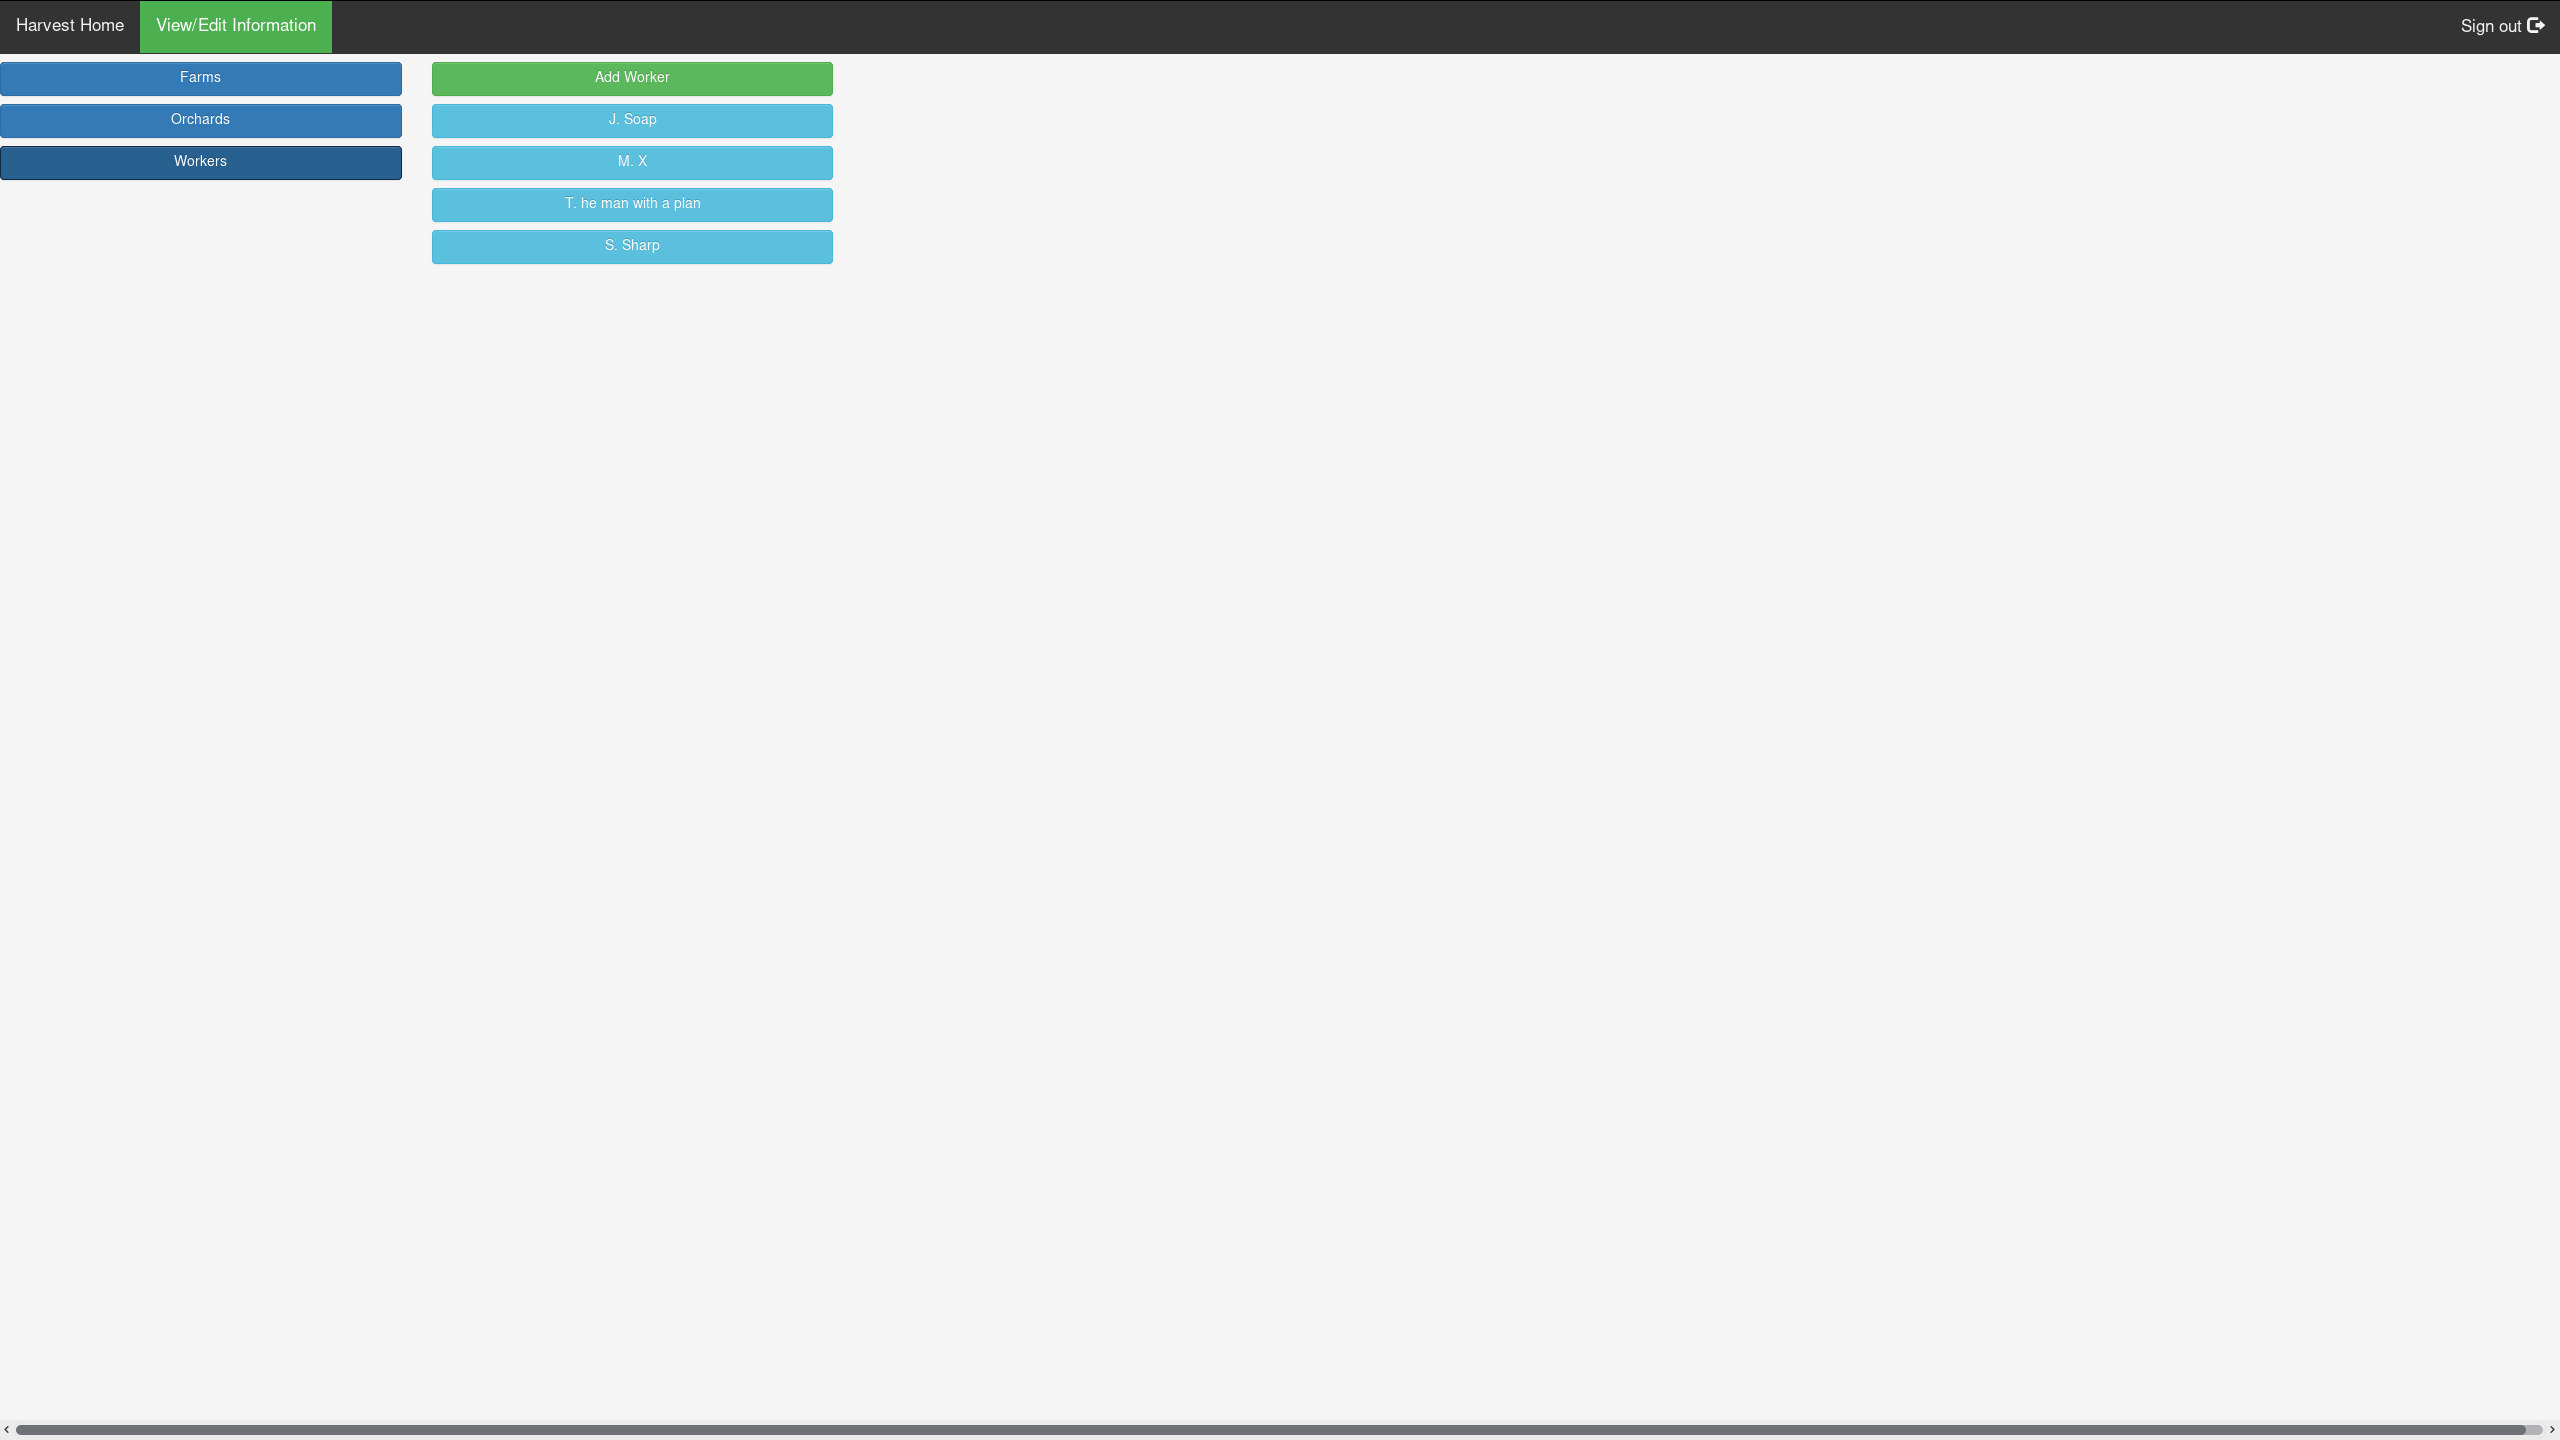
\includegraphics[width=12cm, keepaspectratio]{Images/Information-Workers.png}
 % Screenshot_20180407_191730.png: 2600x1480 px, 121dpi, 54.58x31.07 cm, bb=0 0 1547 881
 \caption{Workers}
 \label{InformationPageWorkers}
\end{figure}

\begin{figure}
 \centering
 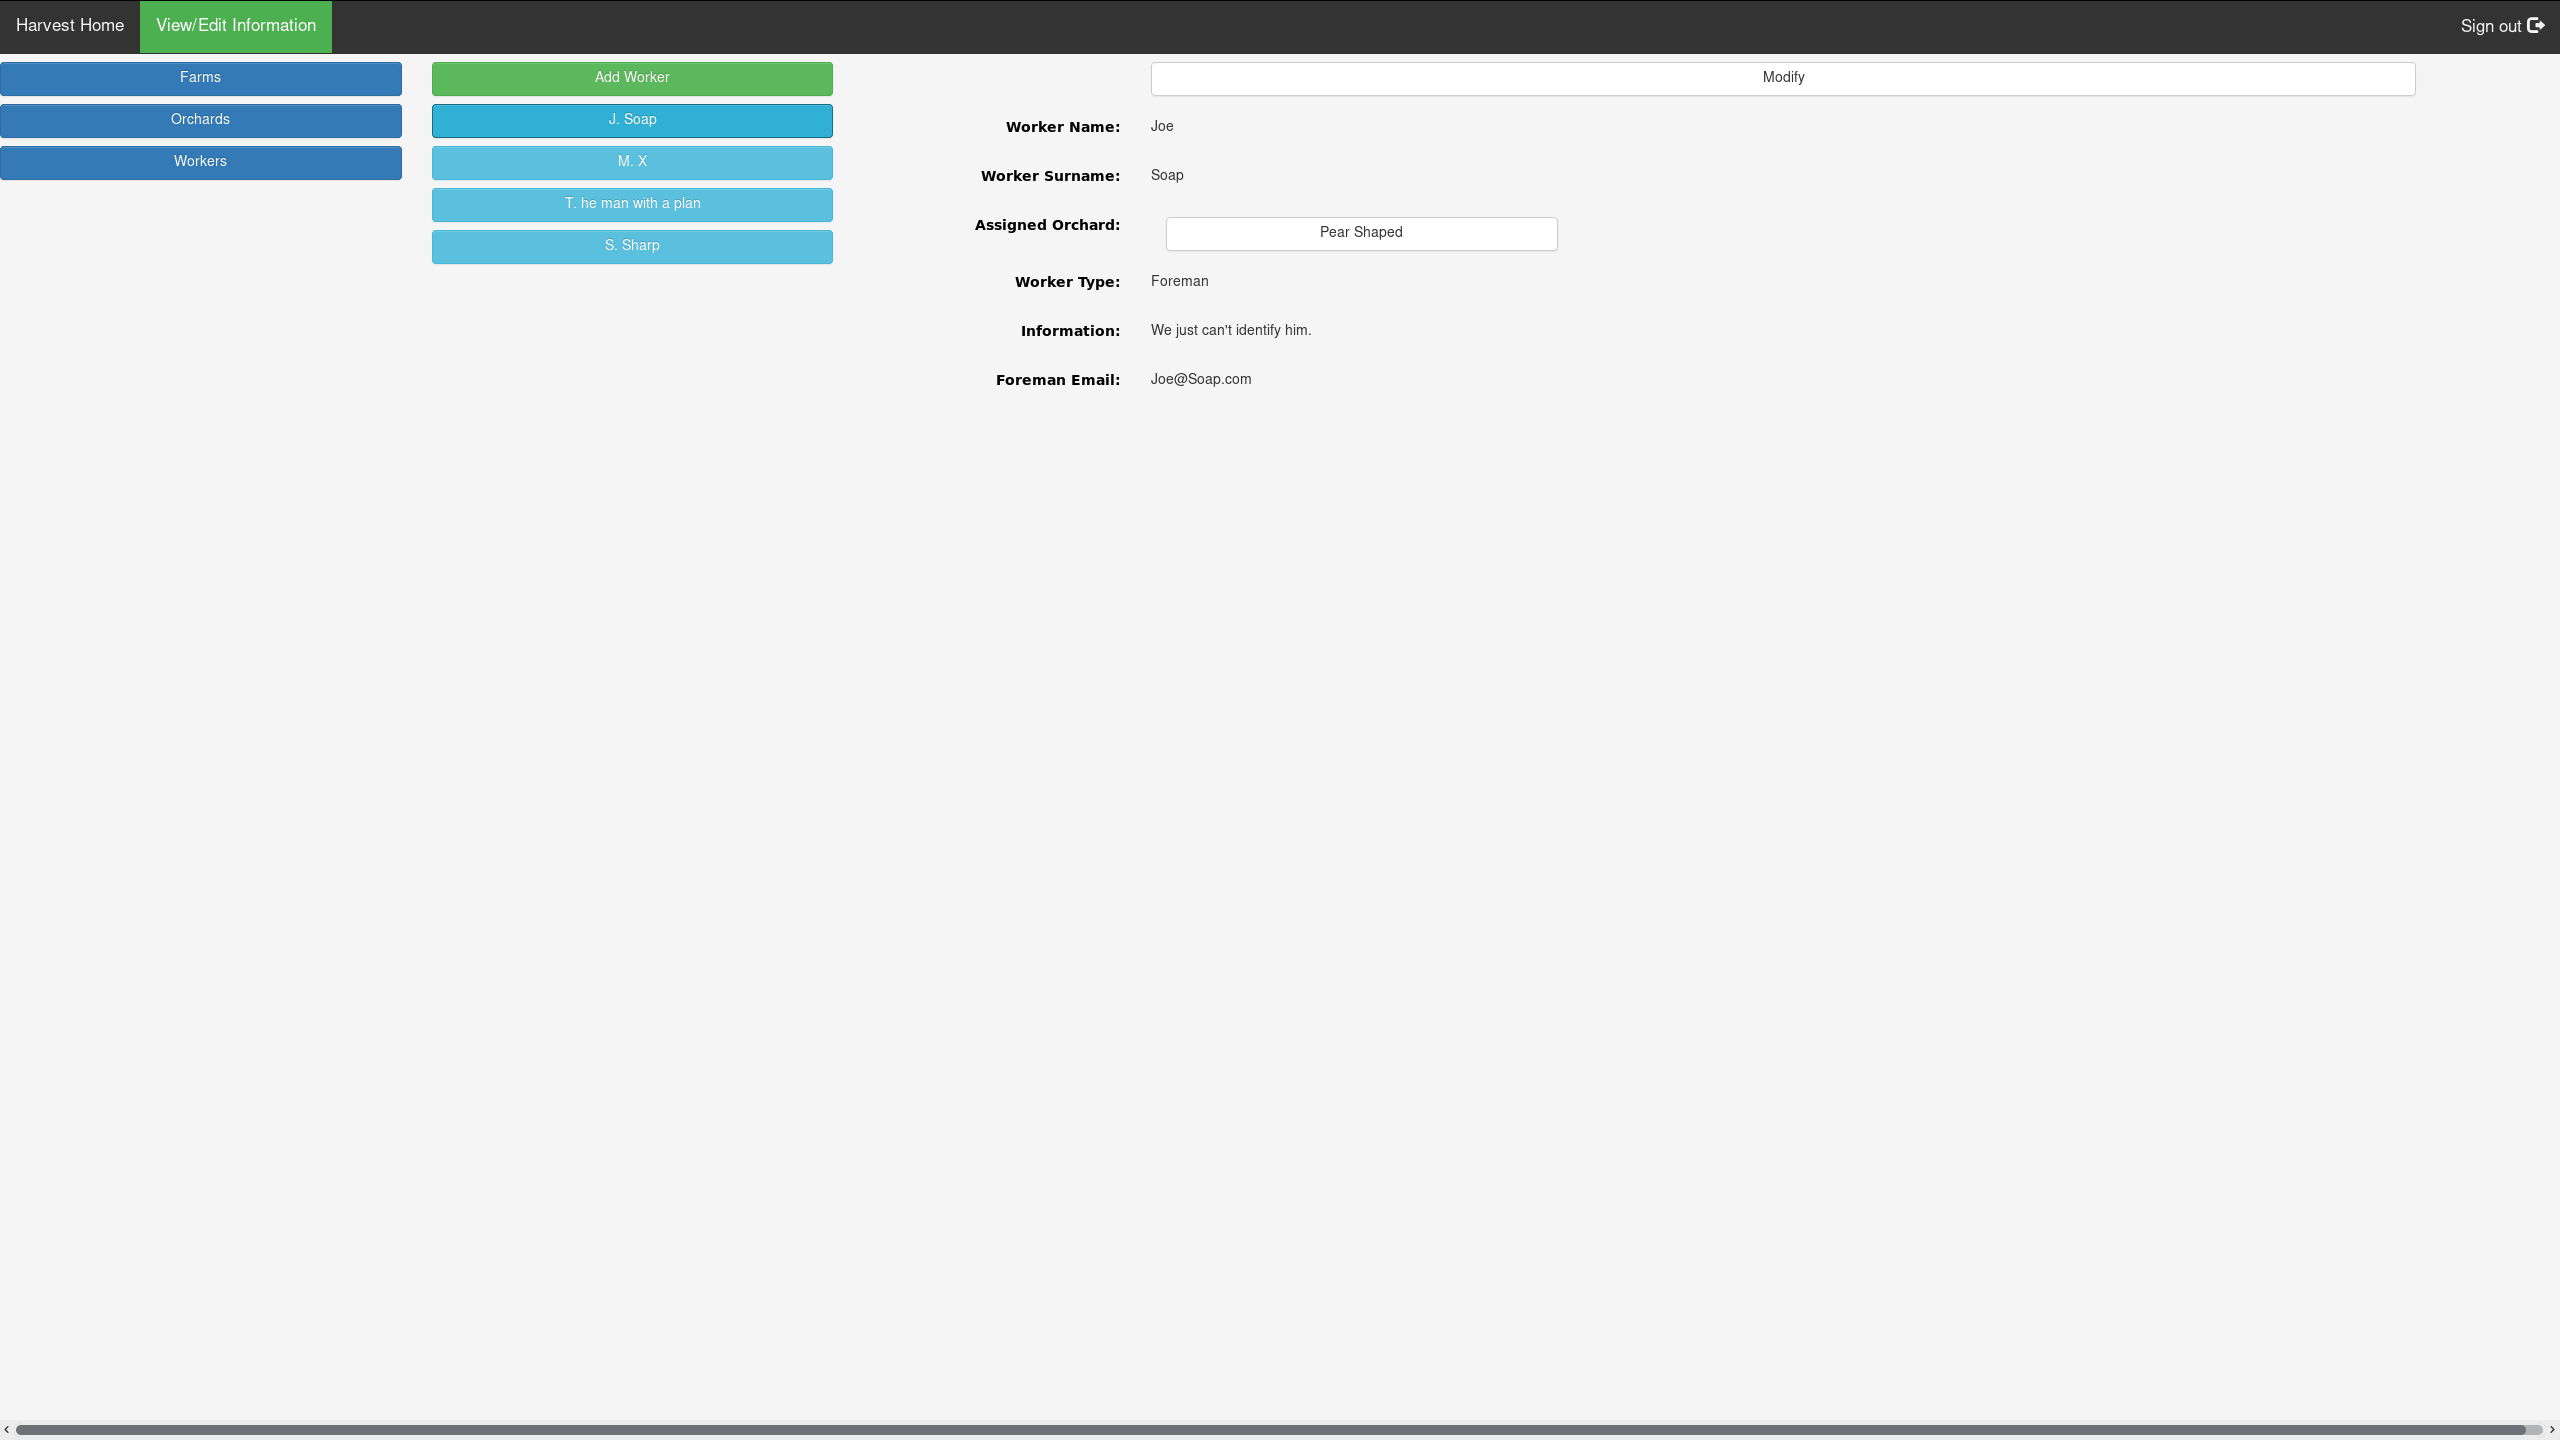
\includegraphics[width=12cm, keepaspectratio]{Images/Information-Joe.png}
 % Screenshot_20180407_191730.png: 2600x1480 px, 121dpi, 54.58x31.07 cm, bb=0 0 1547 881
 \caption{Joe Soap}
 \label{InformationPageJoe}
\end{figure}

\begin{figure}
 \centering
 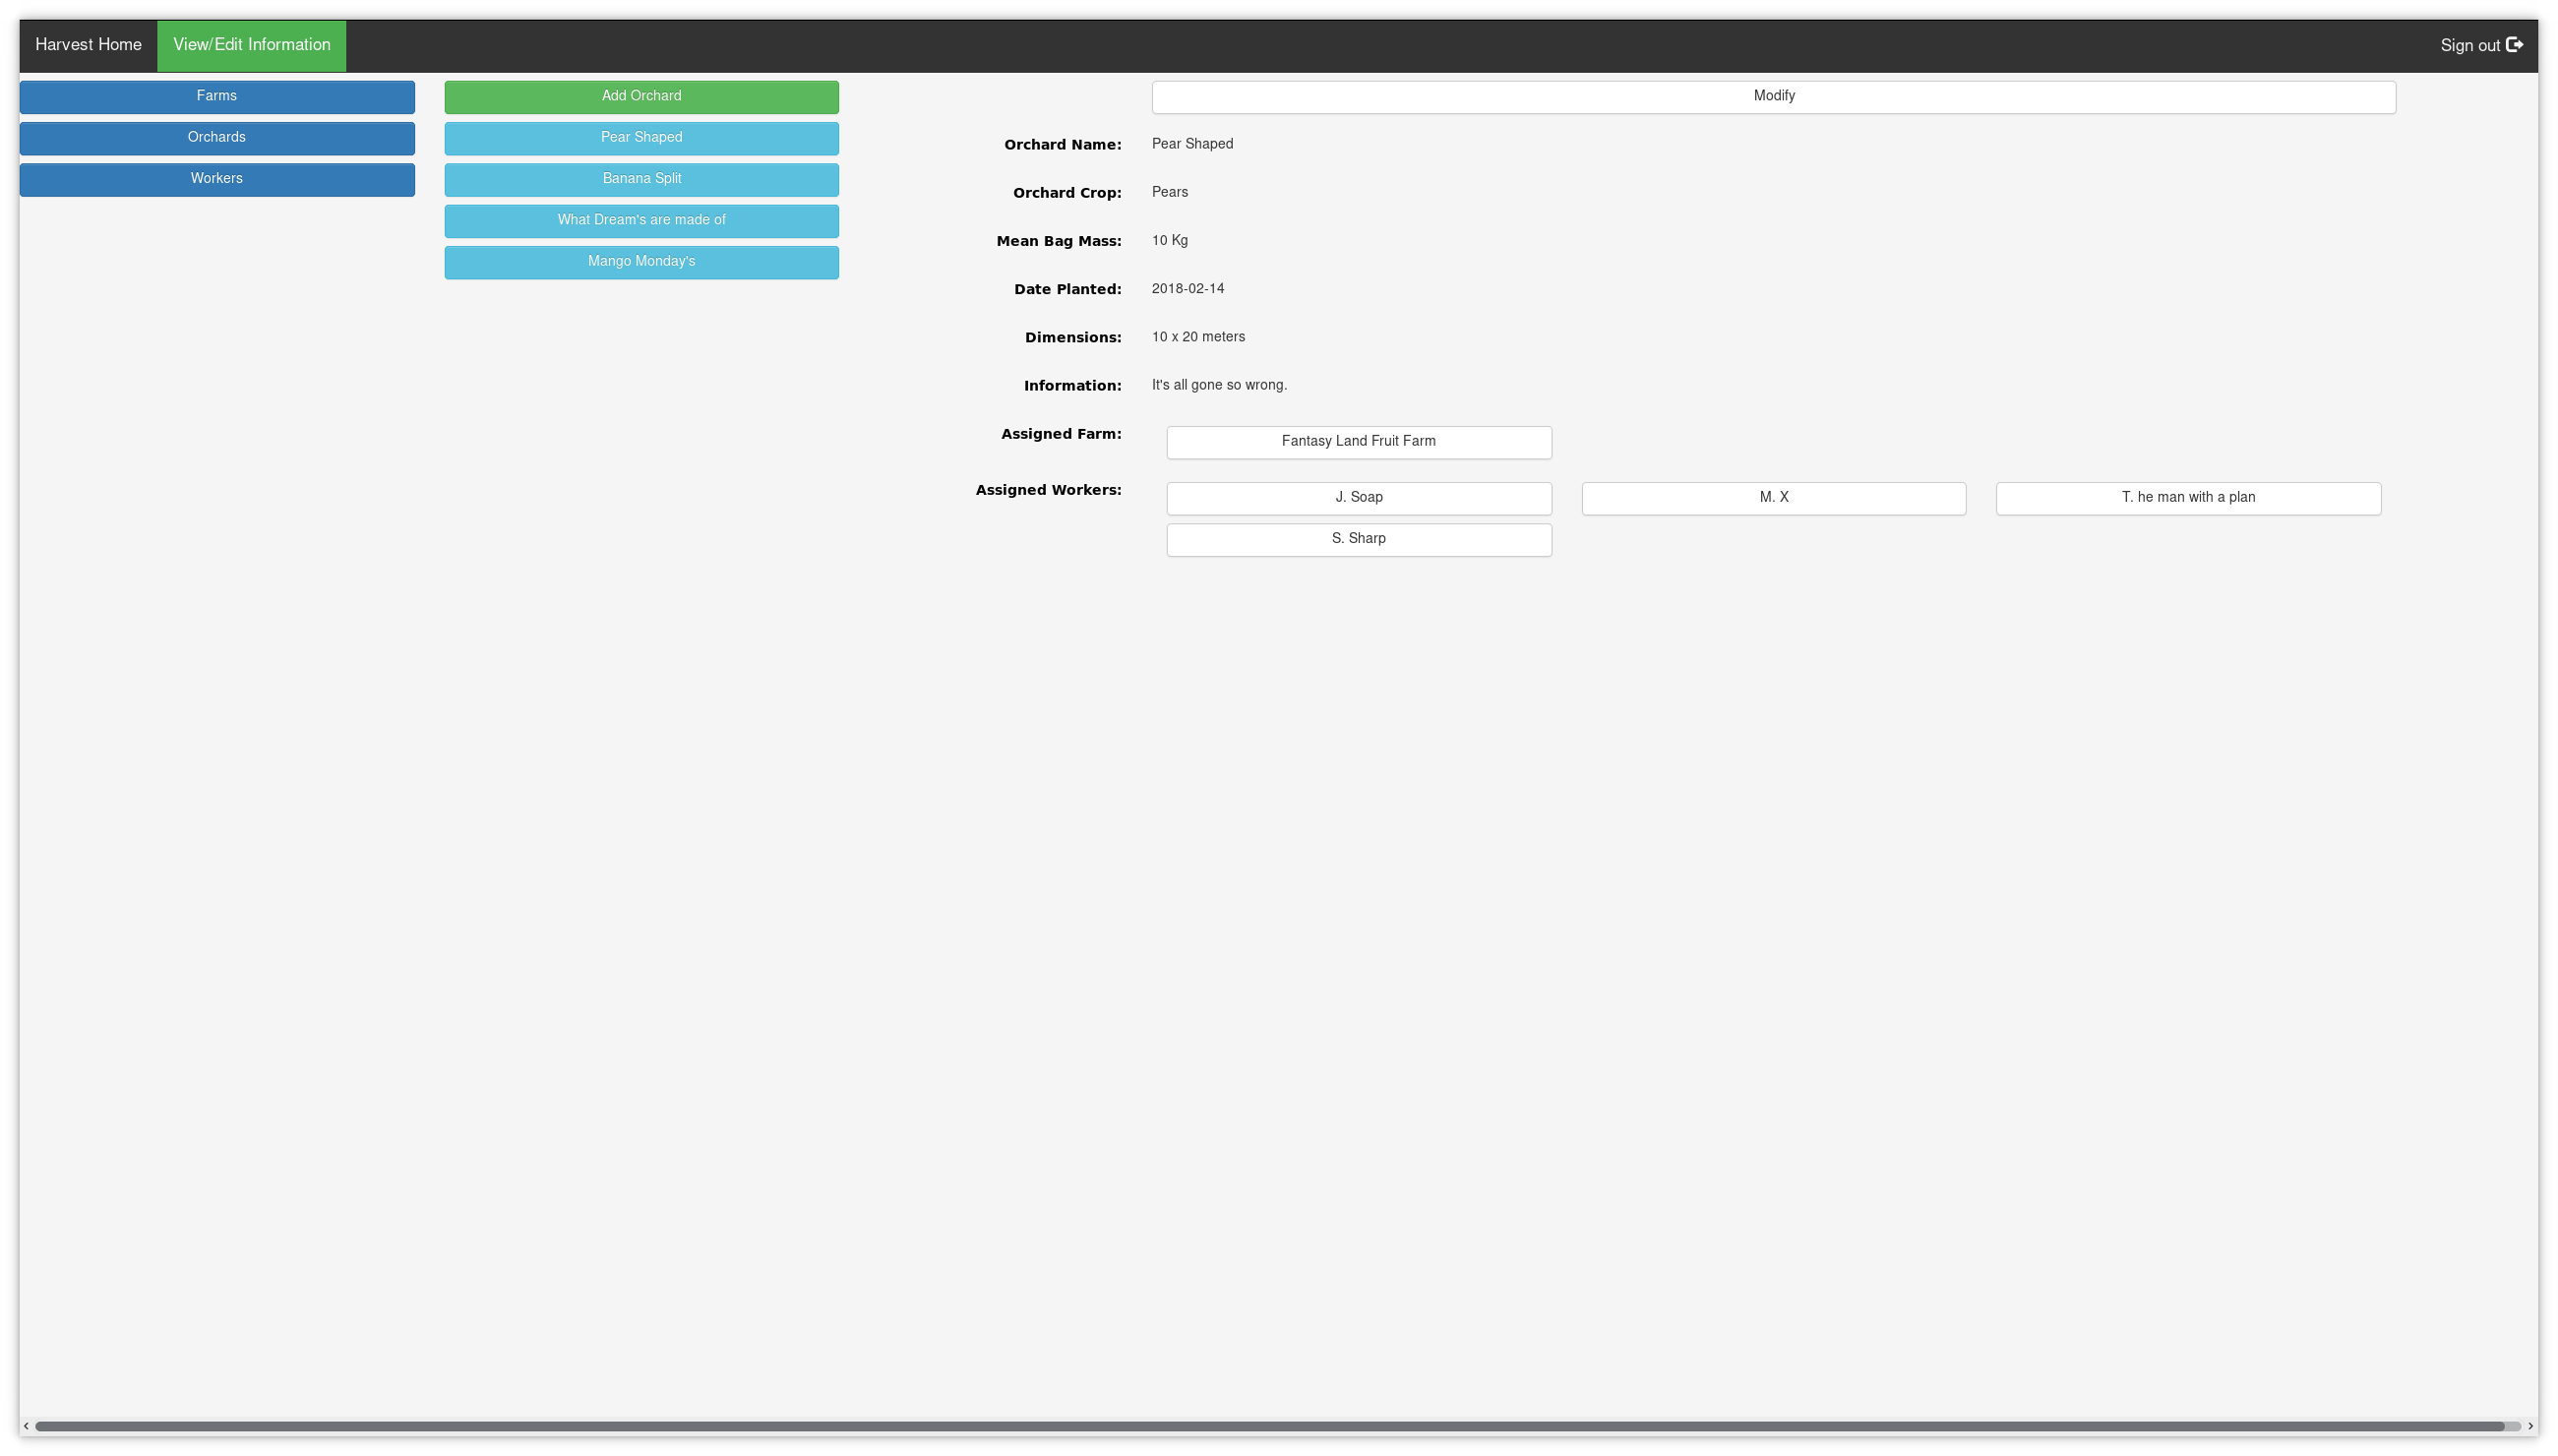
\includegraphics[width=12cm, keepaspectratio]{Images/Information-Pear.png}
 % Screenshot_20180407_191730.png: 2600x1480 px, 121dpi, 54.58x31.07 cm, bb=0 0 1547 881
 \caption{Pear Shaped}
 \label{InformationPagePear}
\end{figure}

\begin{figure}
 \centering
 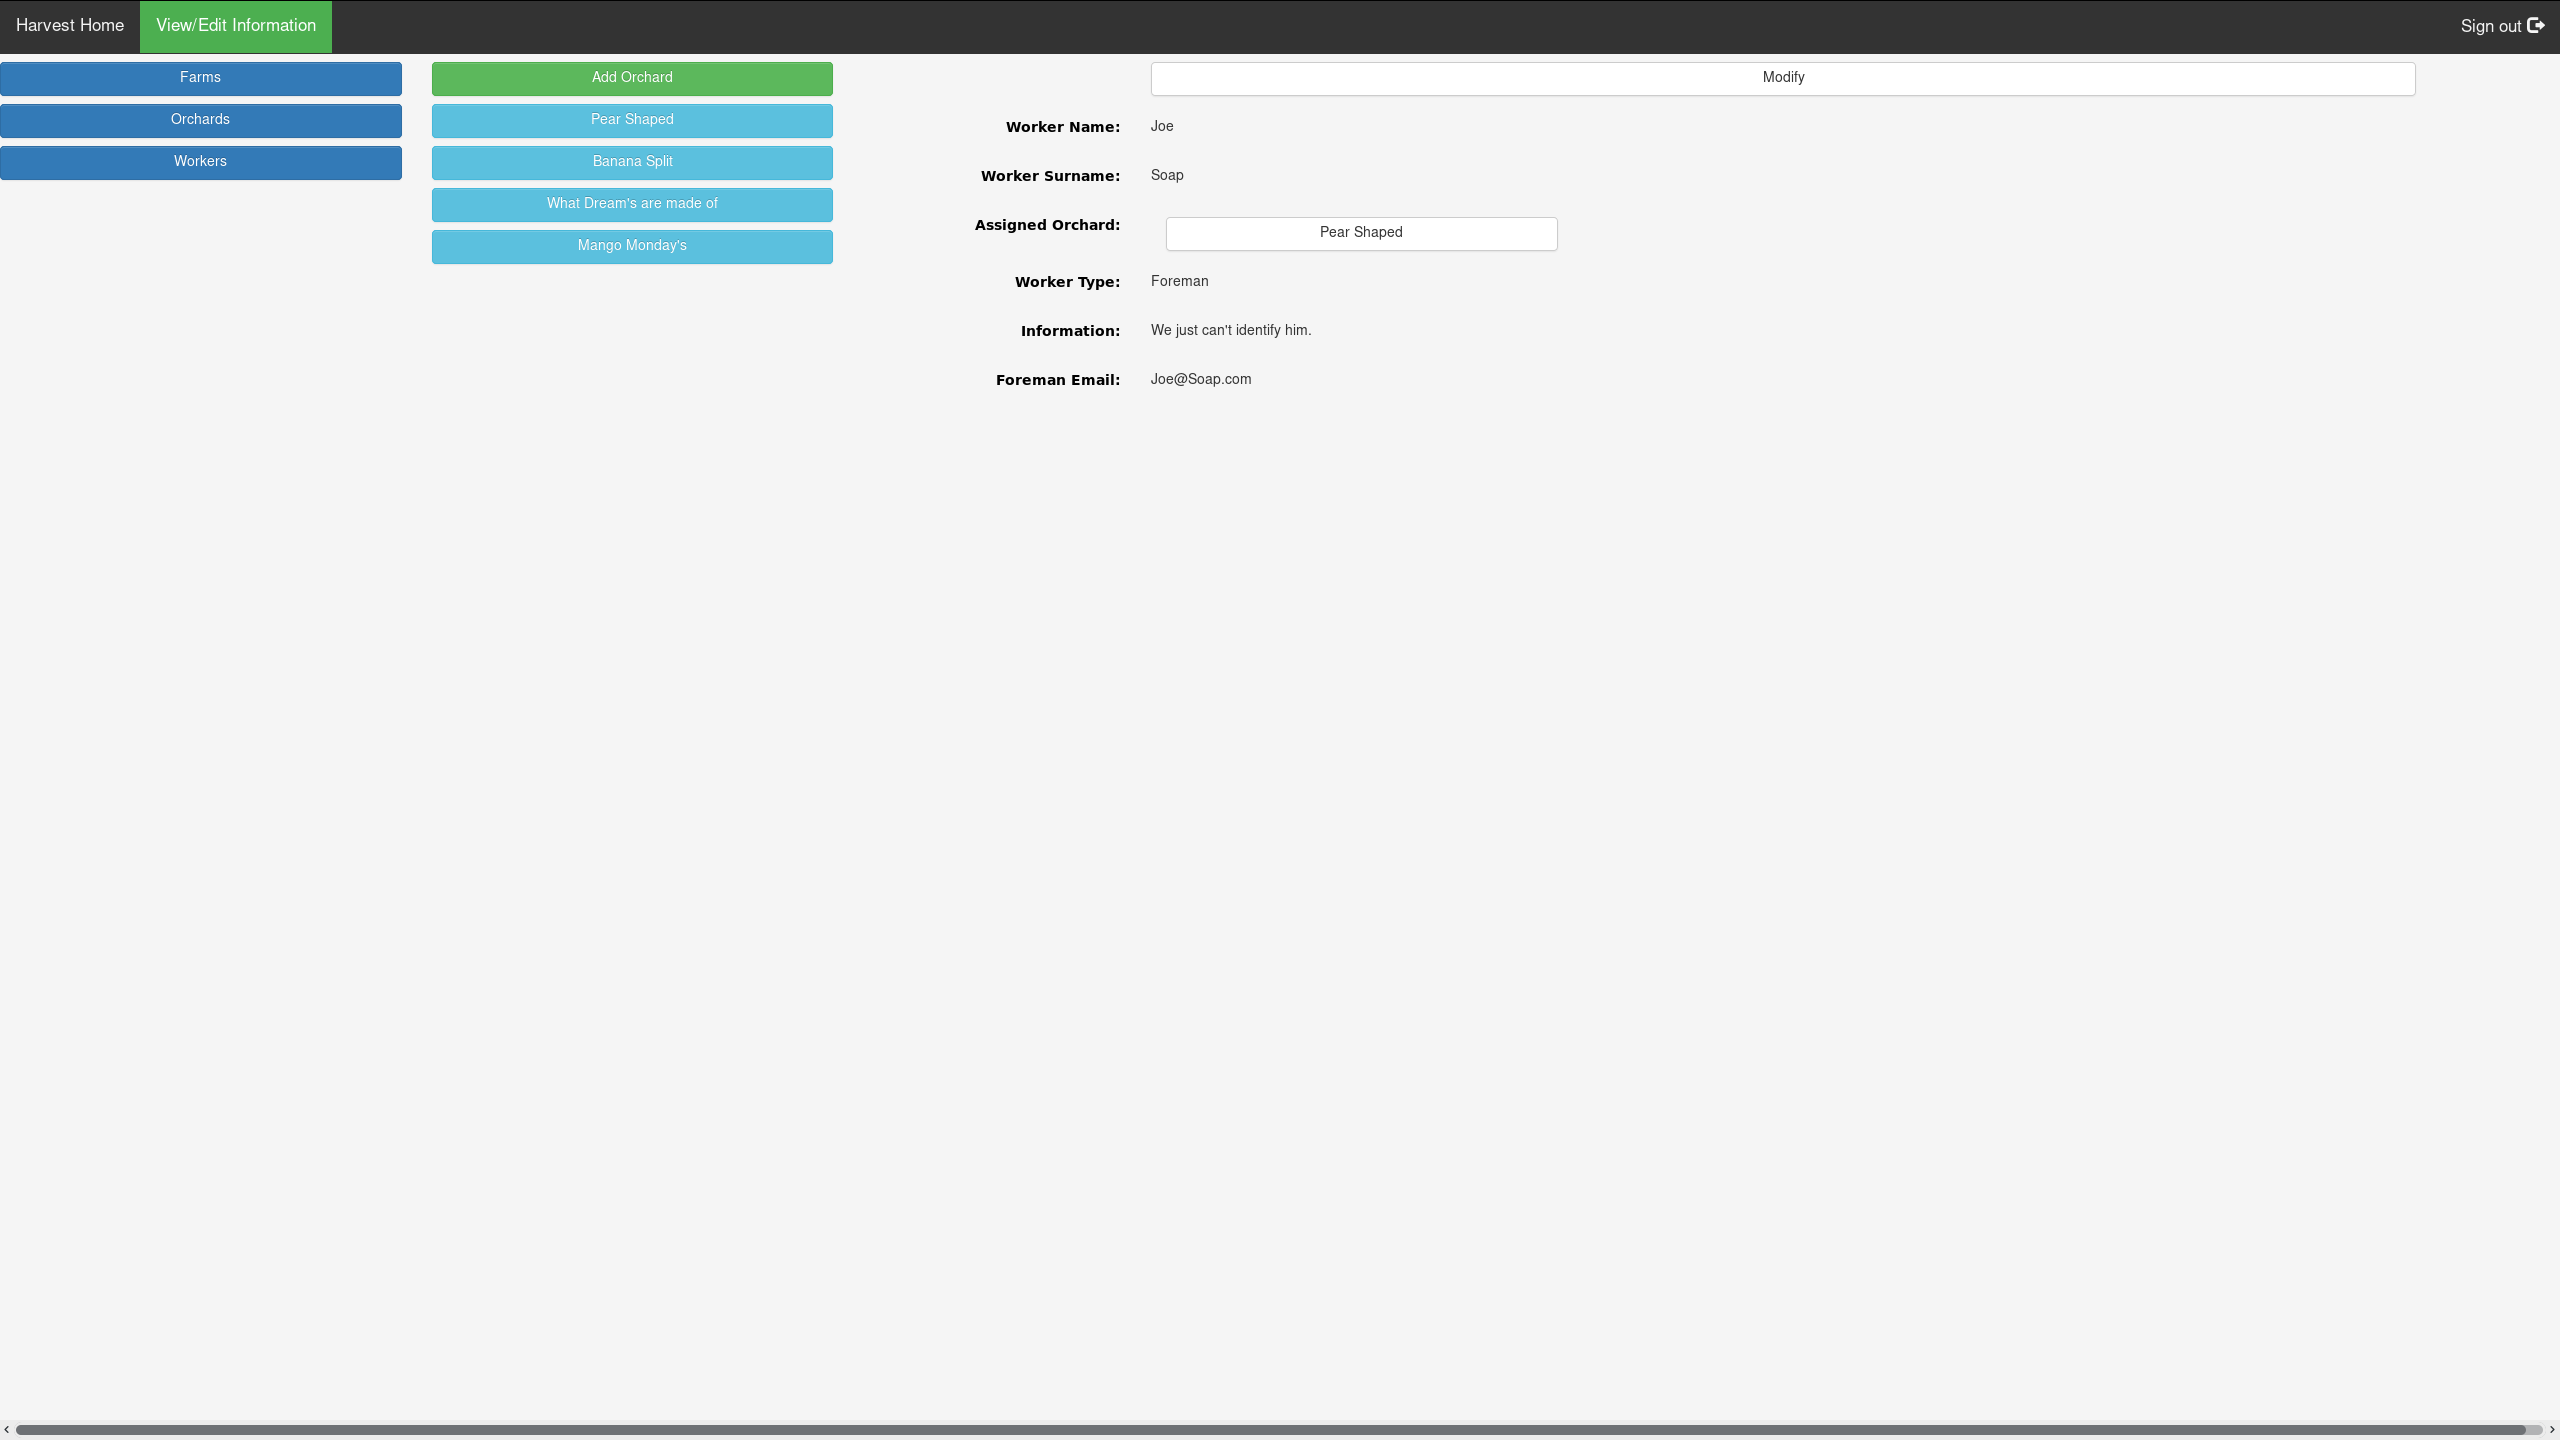
\includegraphics[width=12cm, keepaspectratio]{Images/Information-Joe-Pear.png}
 % Screenshot_20180407_191730.png: 2600x1480 px, 121dpi, 54.58x31.07 cm, bb=0 0 1547 881
 \caption{Joe Soap Through Pear Shaped}
 \label{InformationPageJoePear}
\end{figure}

\paragraph{Adding Information}Note that at the top of the second list in \ref{InformationPageWorkers}, \ref{InformationPageJoe}, \ref{InformationPagePear}, or \ref{InformationPageJoePear} there is a green \texttt{Add Farm}, \texttt{Add Orchard}, or \texttt{Add Worker} button, clicking this button will display the interface to enter the necessary information. An example of this can be seen in \ref{InformationAddOrchard}, where a new orchard can be created. Once all of the necessary information has been entered, then the \texttt{Save} button can be clicked to create the new orchard, note that none of the fields are required.

\begin{figure}
 \centering
 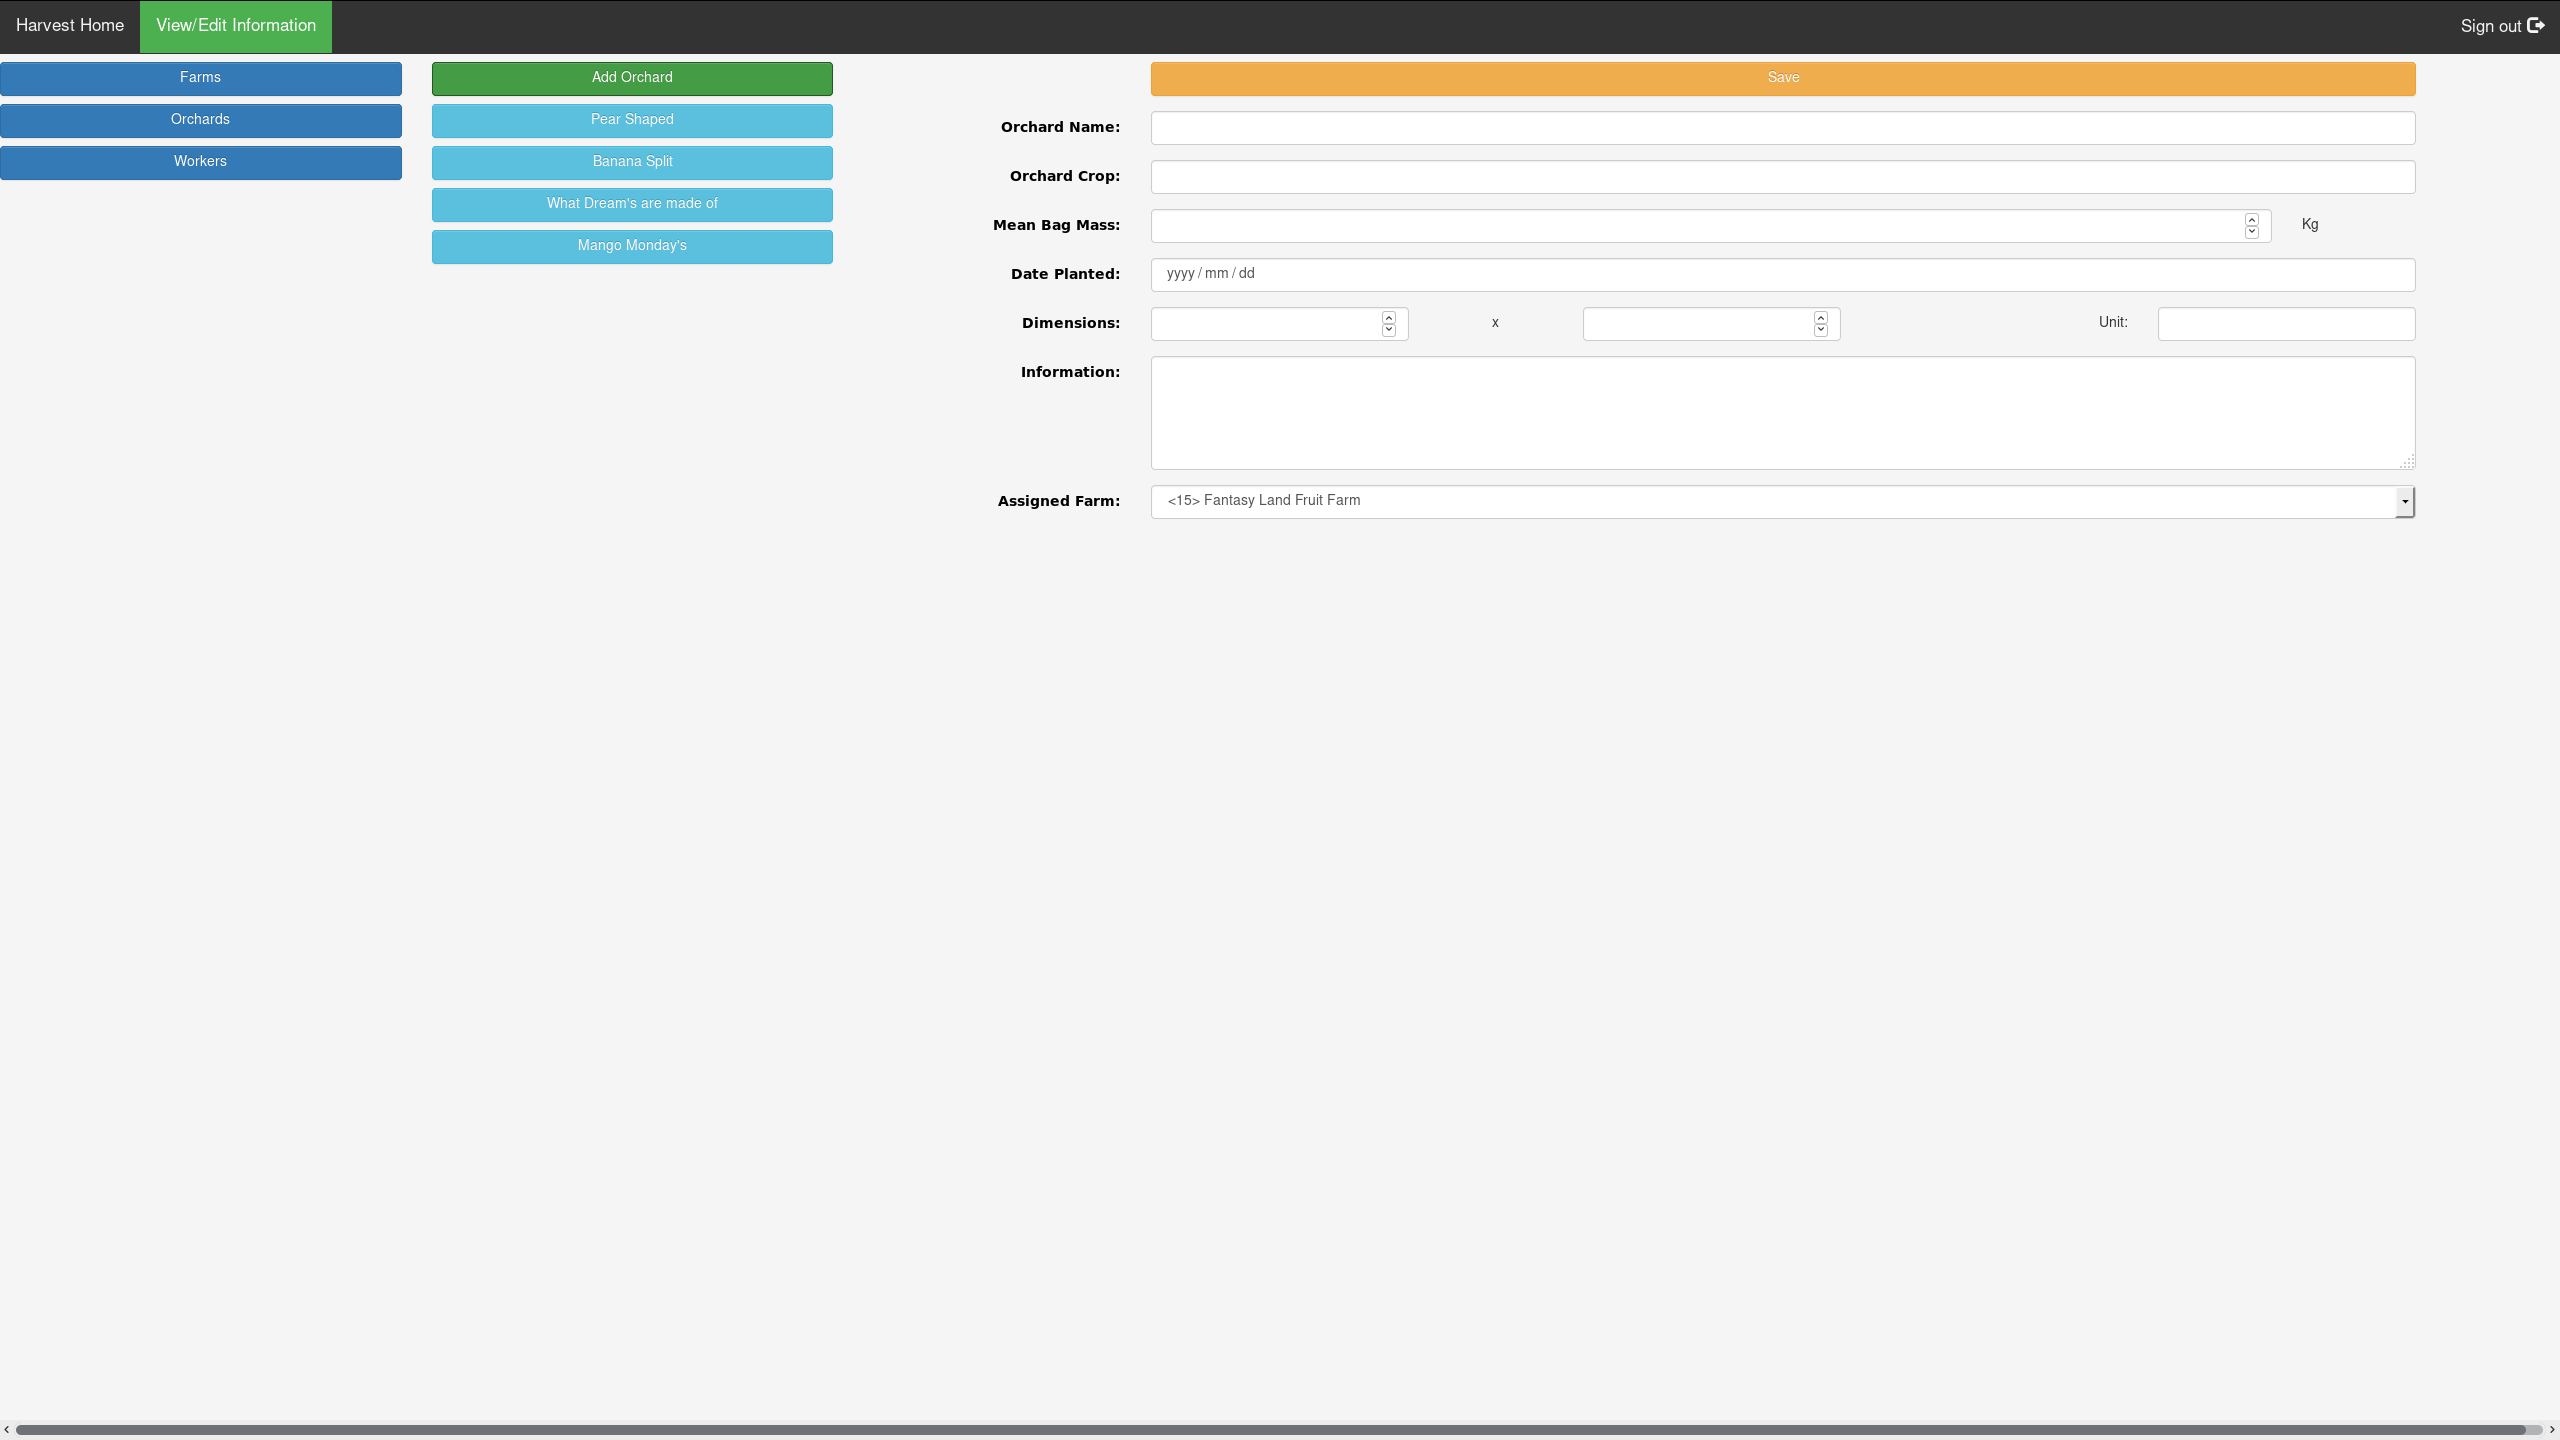
\includegraphics[width=12cm, keepaspectratio]{Images/Information-AddOrchard.png}
 % Screenshot_20180407_191730.png: 2600x1480 px, 121dpi, 54.58x31.07 cm, bb=0 0 1547 881
 \caption{Adding an Orchard}
 \label{InformationAddOrchard}
\end{figure}

\paragraph{Modifying Information}When looking at any information, a \texttt{Modify} button can be seen at the top (see \ref{InformationPageJoe}, \ref{InformationPagePear}, or \ref{InformationPageJoePear}). In \ref{InformationModJoe} the view when \textit{Joe Soap} is being modified can be seen. The fields are already populated by the information that was already stored in them. Once the user is content with the changes, they can click on the orange \texttt{Save} button to apply the changes. A reminder that no fields are required, so that fulled in fields can be erased. The user can also click on the red \texttt{Delete} button to delete the entry in its entirety---note a confirmation dialog will appear. The user may also cancel, which will return them to before they clicked on \texttt{Modify}, as seen in \ref{InformationPageJoe}, \ref{InformationPagePear}, or \ref{InformationPageJoePear}.

\begin{figure}
 \centering
 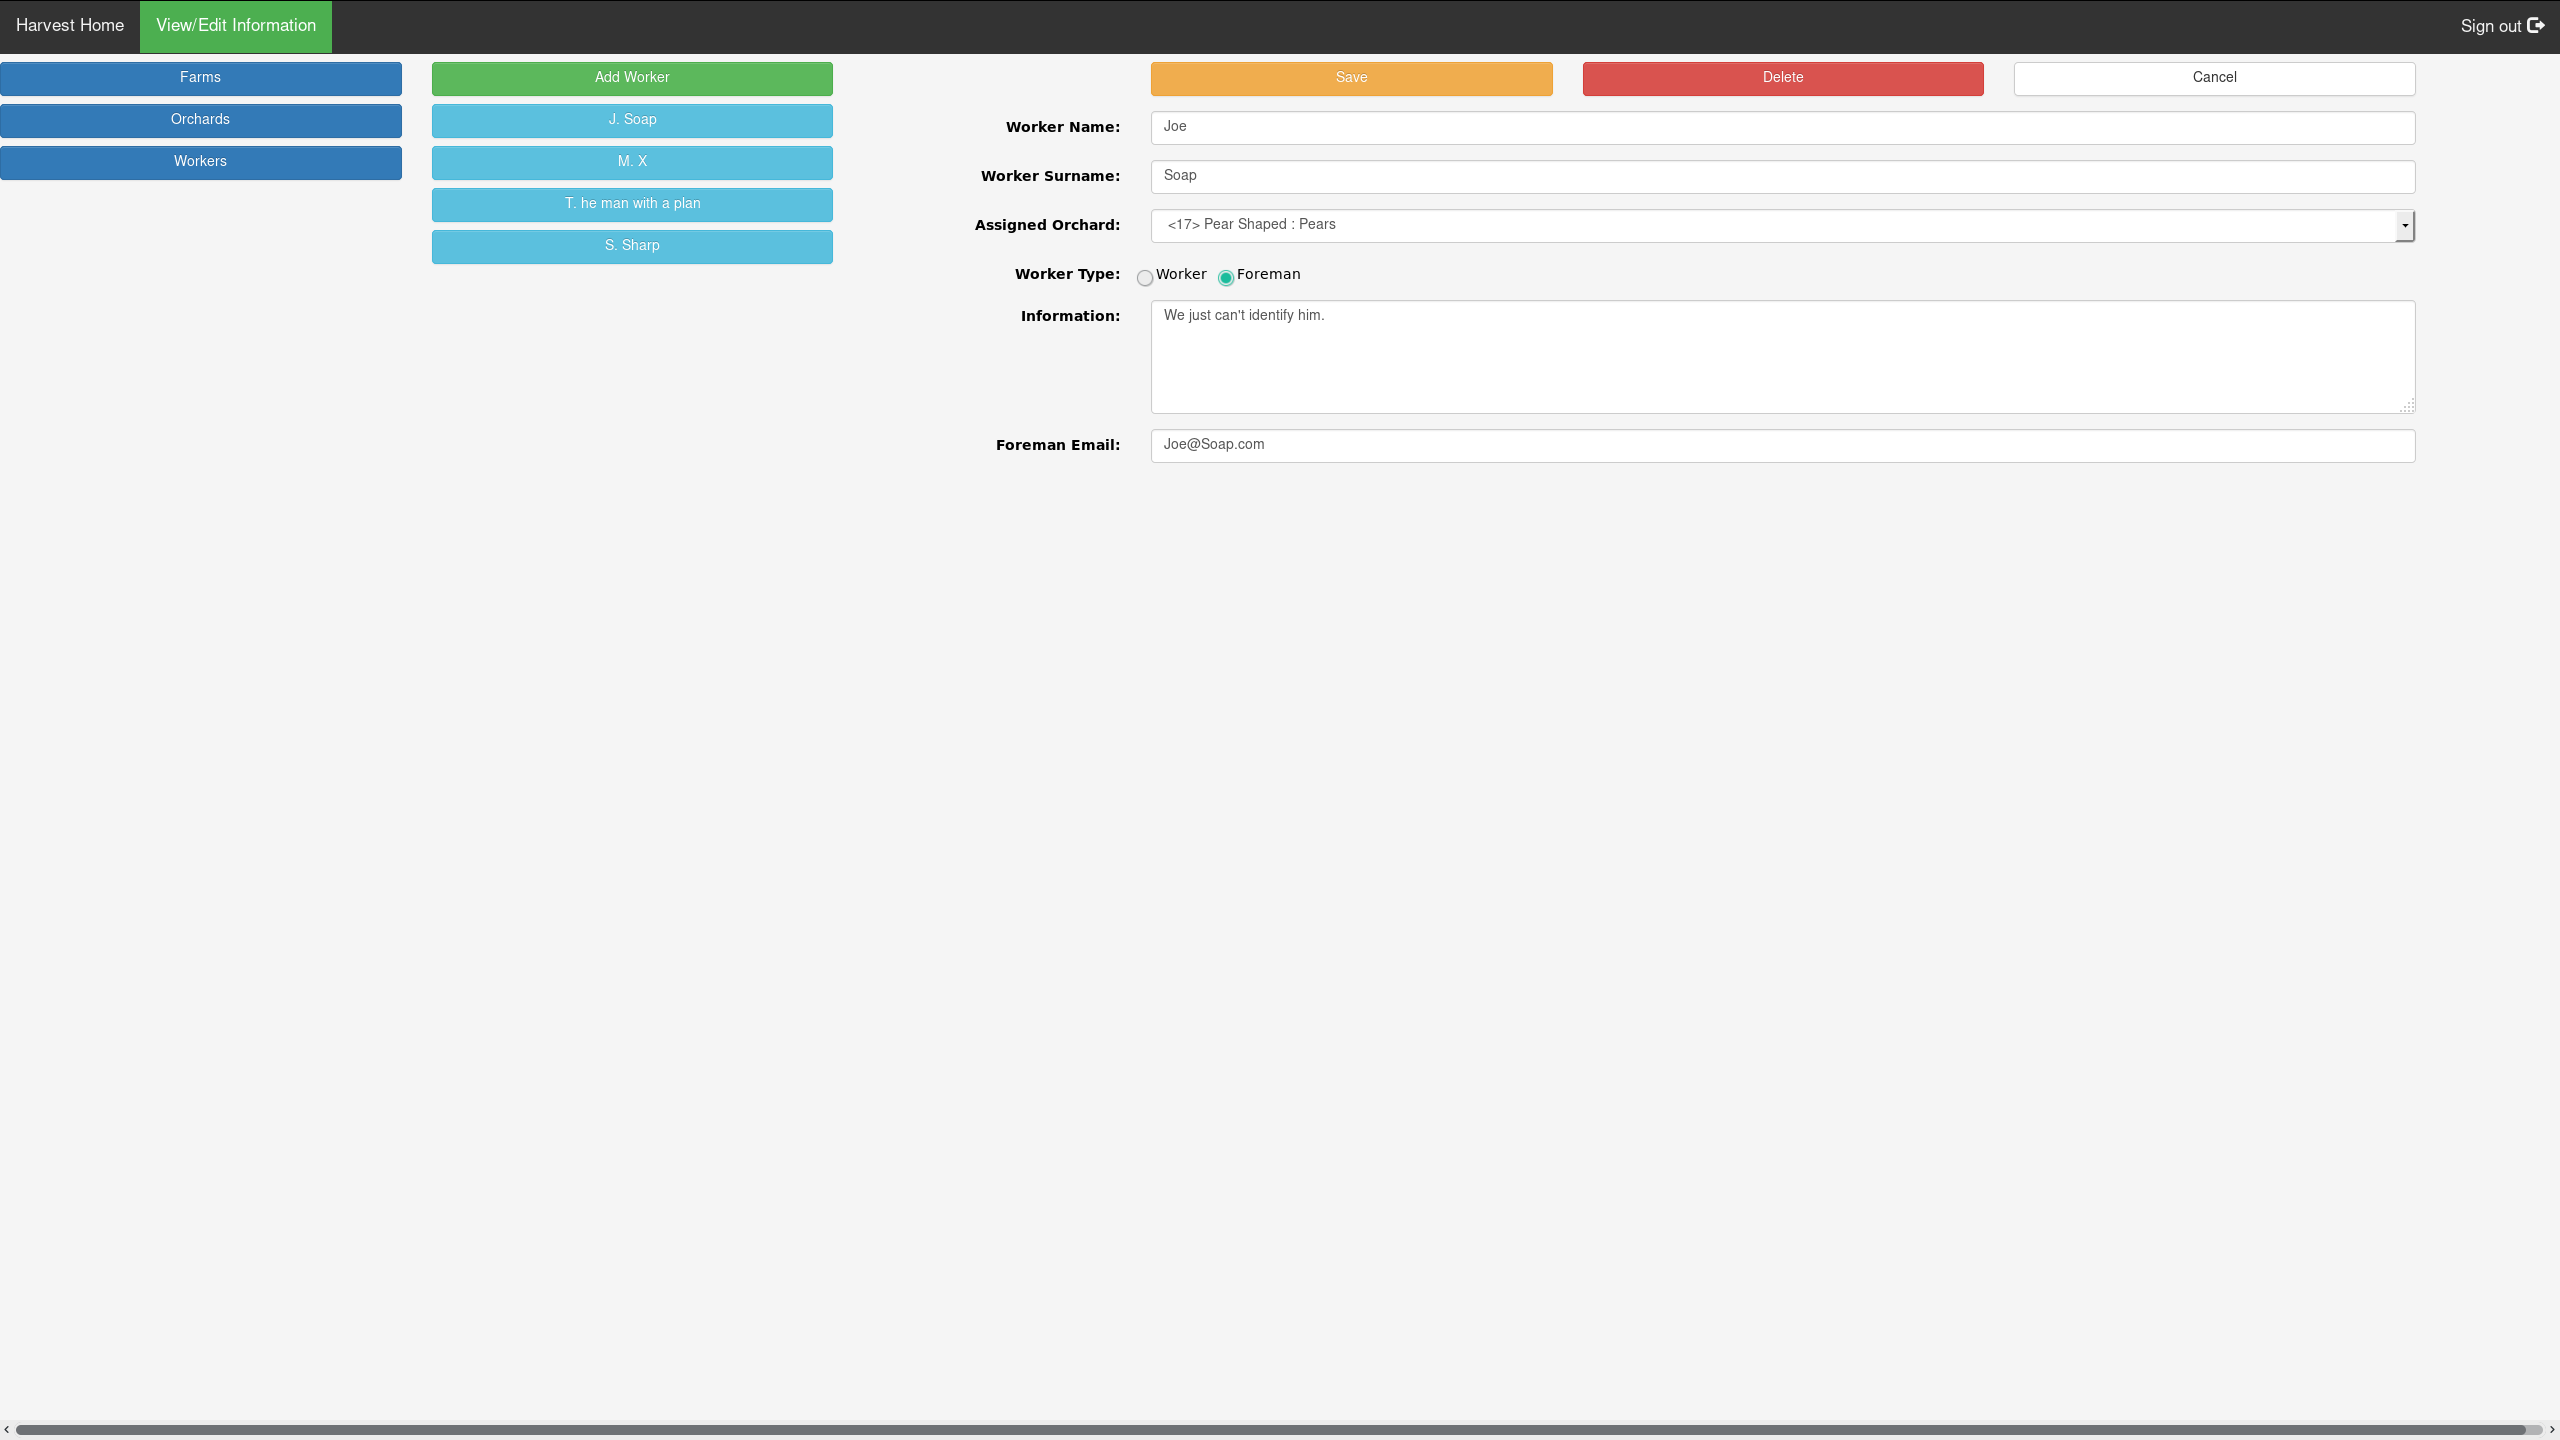
\includegraphics[width=12cm, keepaspectratio]{Images/Information-Mod-Joe.png}
 % Screenshot_20180407_191730.png: 2600x1480 px, 121dpi, 54.58x31.07 cm, bb=0 0 1547 881
 \caption{Modifying Information}
 \label{InformationModJoe}
\end{figure}

\subsection{Stored Information}
Below, the fields stored are described.
\paragraph{Farm}
\subparagraph{Farm Name}The name of the farm.
\subparagraph{Information}Any further textual information about the farm.
\subparagraph{Assigned Orchards}A clickable list of the orchards assigned to the farm.
\paragraph{Orchard}
\subparagraph{Orchard Name}The name of the orchard.
\subparagraph{Orchard Crop}The type of crop grown in the orchard.
\subparagraph{Mean Bag Mass}The average mass of a bag that is harvested from the orchard.
\subparagraph{Date Planted}The date that the orchard was planted.
\subparagraph{Spacing}The spacing of the crops.
\subparagraph{Information}Any further textual information about the orchard.
\subparagraph{Assigned Farm}A clickable button indicating the farm that the orchard is assigned to.
\subparagraph{Assigned Workers}A clickable list of the workers assigned to the orchard.
\paragraph{Worker}
\subparagraph{Worker Name}The first name of the worker.
\subparagraph{Worker Surname}The surname of the worker.
\subparagraph{Assigned Orchard}A clickable button indicating the orchard that the worker is assigned to.
\subparagraph{Worker Type}Indicates if the worker is a foreman or a regular worker.
\subparagraph{Information}Any further textual information about the worker.
\subparagraph{Foreman Email}In the case of a foreman, their email address for linking to their app.





\section{Configuration}
\end{document}
